%%%%
% Consiglio la visione dei seguenti tutorial:
% - https://www.youtube.com/watch?v=ihxSUsJB_14
% - https://www.youtube.com/watch?v=XTFWaV55uDo
%%%%
\documentclass[12pt,a4paper,openright,twoside,draft]{book} % TODO: togliere draft
\usepackage[utf8]{inputenc}

%\newcommand{\thesislang}{italian} % Italian thesis
\newcommand{\thesislang}{english} % English thesis
\usepackage{thesis-style}
% version
\newcommand{\versionmajor}{0}
\newcommand{\versionminor}{1}
\newcommand{\versionpatch}{2}
\newcommand{\version}{\versionmajor.\versionminor.\versionpatch}
\typeout{Document version: \version}

\begin{document}

\frontmatter

% ! TeX root = thesis-main.tex
\title{Title}
\author{Candidate Name Here}
\date{\today}

\newgeometry{margin=0.8in}
\begin{titlepage}
	\begin{center}
		% \vspace*{0.2cm}

		\large
		\textbf{ALMA MATER STUDIORUM -- UNIVERSITÀ DI BOLOGNA \\ CAMPUS DI CESENA}
		\\
		\noindent\hrulefill
		\vspace{0.4cm}

		\Large
		Scuola di Ingegneria e Architettura \\
		Corso di Laurea Magistrale in Ingegneria e Scienze Informatiche

		\Huge
		\vspace{4cm}
		\textbf{
			Design and implementation of a portable Framework for application decomposition and deployment in Edge-Cloud Systems
		}

		\large
		\vspace{1cm}
		Tesi di laurea in
		\\
		\textsc{Pervasive Computing}

		\vspace{5.5cm}
		\begin{minipage}[t]{0.64\textwidth}
			\begin{flushleft}
				\textit{Relatore}
				\\
				\textbf{Prof.} \textbf{Mirko Viroli}
				\\
				\vspace{0.4cm}
				\textit{Correlatore}
				\\
				\textbf{Prof.} \textbf{Danilo Pianini}
			\end{flushleft}
		\end{minipage}
		\begin{minipage}[t]{0.34\textwidth}
			\begin{flushright}
				\textit{Candidato}
				\\
				\textbf{Nicolas Farabegoli}
			\end{flushright}
		\end{minipage}\\

		\vfill
		\noindent\hrulefill
		\vspace{0.3cm}
		\Large

		Quarta Sessione di Laurea
		\\
		Anno Accademico 2022-2023
	\end{center}
\end{titlepage}
\restoregeometry

\begin{abstract}
	Max 2000 characters, strict.
\end{abstract}

\begin{dedication} % this is optional
	Optional. Max a few lines.
\end{dedication}

\begin{acknowledgements} % this is optional
	Optional. Max 1 page.
\end{acknowledgements}

%----------------------------------------------------------------------------------------
\tableofcontents
\listoffigures     % (optional) comment if empty
\lstlistoflistings % (optional) comment if empty
%----------------------------------------------------------------------------------------

\mainmatter

% Introduction --------------------------------------------------------------------------
\chapter{\introductionname}
\label{chap:introduction}
%----------------------------------------------------------------------------------------

With the Internet of Things (IoT), more and more devices are connected to the network producing a very large amount of data.
Cloud computing has been established as a technology for acquiring computational power and storage in support of various applications;
however, it is not always suitable for handling all kinds of systems' requirements: latency, security, and privacy are some of the main
concerns. This comes true especially with IoT systems since they produce lots of data and in some scenarios, they must respect real-time constraints.
For these reasons, fog computing tries to overcome the cloud's limitation by defining a computing model that sits between IoT devices and the cloud.
It allows for the collection, aggregation, and processing of data from IoT devices (or more in general edge devices) using a hierarchy of computing
power.
The combination of fog computing with the cloud can reduce data transfers and communication bottlenecks to the cloud, and can also contribute to
reduced latencies since fog computing resources are closer to the edge.

Nevertheless, realizing systems that operate in the edge-cloud continuum is an open challenge~\cite{BITTENCOURT2018134}:
the heterogeneity of the devices combined with the dynamic nature of the requirements that modern systems must have, leveraging the flexibility of
the edge-cloud continuum is found to be as strategic as it is complex.

Different approaches have been proposed to address the challenges of realizing systems that well interoperate in heterogeneous
infrastructures. Some notable methodologies and frameworks are represented by the osmotic computing paradigm~\cite{8781958}, DR-BIP and its
extensions~\cite{10.1007/978-3-030-03424-5_20,10.1007/978-3-642-30564-1_1,de2020dream}.
While the first approach is mainly oriented to distributed microservices, the latter is more focused on the orchestration of distributed
applications by dynamically adapting the system to the changing requirements basing the systems on the \emph{motif} concept.

In the CPS context, engineering systems featuring distributed intelligence in a \emph{self-organization} fashion is one of the main relevant
approaches. In this way, the global behaviour of the system is obtained by the interaction of the individual components giving robustness to the
system. The current trend of large-scale, dynamic and heterogeneous Cyber-Physical Systems requires increasingly complex and diverse
infrastructures. Remote clouds offer a seemingly supply of computing, storage, and services on demand, but this comes with the caveat of high
costs and potential latency issues, as well as data protection concerns that must align with the specific requirements of each application. Edge
computing, on the other hand, brings resources closer to users, resulting in reduced latency and increased reactivity, while simultaneously
addressing data dissemination concerns.

As stated before, such infrastructures are not easy to manage and orchestrate, complicating the engineering phase where the logic of the
system tends to be coupled with infrastructure aspects. Generally, this prevents the reusing of design elements across different scenarios by
exploiting the underlying infrastructure opportunistically.

To tackle this problem the \emph{pulverization approach} is proposed~\cite{fi12110203}: this framework brakes the system behaviour into small
computational pieces logically linked to sensors and actuators that are continuously executed and scheduled in the available infrastructure.
In this way, the system can be seamlessly mapped onto a variety of multi-layered deployment infrastructures.
It is based on a flexible logical model which can be decomposed into a set of sub-components with well-defined relationships that can be deployed and 
wired separately. The pulverization facilitates the deployment independence of a system, namely the ability to run the application with no change
on various deployments retaining its original functional semantics.
In this way, the application logic will obtain the functional goals independently of the actual deployment since the choice of the deployment 
strategy is affected typically by non-functional requirements such as latency, security, performance and cost.
This approach is formalized to provide an unambiguous specification of what constitutes pulverization by clarifying subtle aspects of the model
and state the deployment-independence property rigorously. 

The main contribution of this thesis is the development of a framework that leverages the pulverization approach to orchestrate distributed
applications in the edge-cloud continuum.
This framework aims to lay the groundwork for closing the gap between the simulation of these systems and their deployment by exploiting the
pulverizing methodology.
Although the pulverization approach originates in the context of aggregate computing, the framework aims to be generic enough to enable the
pulverization in non-aggregate systems as well.
To showcase the effectiveness of the framework, some scenarios in the context of CPS have been identified by using the framework to deploy such
systems, highlighting the potential that pulverization has as a methodology.
In particular, the framework is used in conjunction with \emph{embedded systems} to recreate a heterogeneous infrastructure where the framework
runs on.

%
\paragraph{Thesis Structure.} % Optional paragraph title
%
Accordingly, the remainder of this thesis is structured as follows.
%
\Cref{chap:background} discusses the background and related works.
%
\Cref{chap:requirements} summarize the requirements of the framework and give an overview of relevant deployment scenarios that are worth
to be considered during the validation of the framework.
%
\Cref{chap:design} presents the framework and its architectural design.
%
\Cref{chap:implementation} describes the implementation details of the framework.
%
\Cref{chap:validation} shows the validation process of the framework, including the experimental setup and the results obtained by the demos.
%
Finally, \Cref{chap:conclusions} concludes this thesis by summarizing its main contribution, with a focus on future works.
%----------------------------------------------------------------------------------------

% State of the art ----------------------------------------------------------------------
\chapter{Background}
\label{chap:background}

This chapter is organized into three sections. The first section provides an overview of the current layered and heterogeneous infrastructure
defined by the could-edge interplay. The second section describes the problem of the deployment independence of the applications by giving an
overview of the actual frameworks and methodologies. Finally, the third section describes the pulverization methodology in aggregate computing and
cyber-physical systems.

\section{Layered and heterogeneous infrastructure}
\label{sec:layered-heterogeneous-infrastructure}

Nowadays, electronic devices are capable of generating vast amounts of data, from measuring natural phenomena to human behavior.
The growth of the Internet of Things (IoT) is expected to connect virtually all objects, leading to a need to transfer, store, and process
unprecedented amounts of data.

Cloud computing has become an accessible platform for storing and processing data for a variety of applications, including IoT devices. It offers
flexibility and low initial costs, but its adoption has exposed limitations in fulfilling requirements for real-time, low-latency, and mobile
applications. Centralized cloud data centers are often physically and logically distant from the client, requiring multiple hops and causing delays
and consuming network bandwidth.

The adoption of cloud computing and the increasing ability of edge devices to generate and consume heterogeneous data requires new distributed
computing infrastructures that can handle diverse application requirements. Recent computing infrastructures that enact applications at edge devices
have improved response time and reduced bandwidth use. Fog computing has emerged as a paradigm that combines the ability to run localized
applications at the edge with the high capacity of the cloud, supporting the heterogeneous requirements of both small and large applications through
multiple layers of the computational infrastructure.

Taking advantage of the characteristics of the edge-cloud continuum enables many opportunities in the Internet of Things field, like
having systems that comply with requirements such as security, data locality, real-time computation, etc.
Nevertheless, the deployment of applications in this infrastructure is still a challenge and several approaches have been
proposed to address this issue~\cite{BITTENCOURT2018134}.

In the following section will be provided an overview of the main aspects and challenges that demonstrate the suitability of combining edge, fog,
and cloud computing for various applications used by the Internet of Things.

\subsection{Cloud Fog and Edge interplay}
\label{sec:cloud-fog-edge-interplay}

This section introduces the concepts and terminology of cloud, fog, and edge computing, discussing their main characteristics and finally, how
those paradigms can be combined to provide a more flexible and efficient solution for a wide range of applications.

\subsubsection{Cloud computing}

Over the last decade, cloud computing has become a widely adopted computing paradigm for many applications due to its dynamic characteristics such as elasticity and pay-per-use (achievable via virtualization and containerization), reaching a mature state.

Cloud providers offer on-demand computing through three main models, which are Infrastructure as a Service (IaaS), Platform as a Service (PaaS), and
Software as a Service (SaaS)~\cite{armbrust2010view}. IaaS provides users with remote access to computing power as a service, while PaaS offers a
platform for software development with necessary libraries and databases to deploy and run applications, and SaaS provides software that relies on
cloud providers' infrastructure to offload computing and/or data. The concept of Everything as a Service (XaaS) has emerged, which
includes a wide variety of cloud service levels.

Cloud services operate under a Service Level Agreement (SLA) that determines the services offered and the costs for using them. Common pricing models
include charging by time unit, amount of data transfer, and the number of requests. Cloud computing's features of elasticity, ubiquitous access, and
on-demand provisioning make it an attractive option, allowing for lower upfront investments and faster time to market, with reduced
operational costs.

\subsubsection{Fog computing}

The evolution of hardware in personal devices has increased computing capacity at the edge and the size of mobile devices has shrunk, allowing them
to run applications with reasonable complexity and quality of service (QoS). As a result, distributed computing paradigms are being utilized, where
edge devices are used to run applications and store data.

Fog computing creates a bridge between edge devices and the cloud, and introduces a hierarchy of computing capacity, with fog nodes, cloudlets, or
micro data centers located between the edge and the cloud. This hierarchy can be spread throughout the network, with nodes higher in the hierarchy
having larger computing capacity and serving more users, while nodes lower in the hierarchy are closer to the edge and have lower communication
delays.

The computing hierarchy in the fog infrastructure can offer a wider range of service levels, supporting applications that cannot be supported by
cloud computing alone. A fog infrastructure can handle applications with a variety of QoS requirements, as applications can run at a hierarchy
level that provides adequate processing capacity and meets latency requirements. Another consequence of the use of processing closer to the edge is
to reduce (aggregate) bandwidth use in the network along the path between the edge and the cloud.

\subsubsection{Edge computing}

Edge computing is a distributed computing paradigm that brings computation and data storage closer to where it is needed, reducing the distance that
data must travel and minimizing the latency for applications that require quick responses. Edge computing evolved from the growth of mobile devices
and the hardware evolution of personal devices.

The combination of higher computing capacity and edge networks enabled distributed computing paradigms that propose the utilization of edge devices
to run applications and store data. Edge computing is characterized by the use of devices such as smartphones, tablets, and IoT sensors and actuators
as sources of computational and storage resources. These devices have limited computational capacity and battery life but can support application
execution and storage capabilities.

Edge computing is expected to enable new applications in areas such as augmented reality, autonomous vehicles, and smart cities, among others, by
allowing data processing and analysis to occur closer to the data source, reducing response time and network congestion. Edge computing also enables
the collection of data from a variety of sources and the aggregation of data at the edge for further processing, analysis, and decision-making.

\paragraph*{}

Fog computing and edge computing are two related but distinct concepts in the field of distributed computing. However, they are often used
interchangeably or confused with one another, which can lead to misunderstandings and miscommunication.

One reason for the confusion is that both fog and edge computing refer to distributed computing infrastructures that process data closer to where it
is generated, such as on the edge of the network. They both aim to reduce network latency and bandwidth consumption by processing data locally rather
than sending it to a centralized cloud server.

However, the main difference between fog and edge computing lies in the level of hierarchy at which they operate. Edge computing typically refers to
processing that occurs at the outermost layer of the network, closer to end-user devices and sensors. It involves lightweight computing devices and
microservices that are often embedded in sensors, smartphones, or IoT devices.

Fog computing, on the other hand, involves a hierarchy of computing nodes that are distributed between the edge and the cloud. These nodes, also
known as fog nodes, cloudlets, or micro data centers, can be located at access points, routing devices in the network, or even at the core of the
network. The idea is to provide a distributed infrastructure that can handle data processing and analysis at different levels of the network
hierarchy while minimizing latency and bandwidth usage.

In conclusion, while fog computing and edge computing share similar goals and concepts, they are distinct in their approach and level of hierarchy.

\subsubsection{Edge-cloud continuum problems}

The edge-cloud continuum presents many challenges that must be addressed to optimize its performance. One of the primary issues is
managing the resources distributed across the continuum in a way that ensures efficient resource utilization and maintains QoS levels. This is
particularly challenging due to the heterogeneity of devices and applications that comprise the continuum, as well as the dynamic nature of the
network topology caused by device mobility and varying application requirements.

The movement of services in the Edge-Cloud infrastructure is an important consideration due to the inherent heterogeneity of the devices and
applications in the system. As edge and fog computing become more prevalent, there is a greater need for services to move between devices in the
hierarchy to optimize the use of resources and provide the required Quality of Service (QoS). However, managing the automatic adaptation of
services to different deployment locations while considering resource constraints at each level of the infrastructure is a major
challenge. Additionally, the heterogeneous network topology and frequent changes in device mobility and application requirements make it even more
complex.

% - New section ---------------------------------------------------------------

\section{Deployment independence}
\label{sec:deployment-independence}

The advantages of integrating different computing paradigms, such as cloud and edge computing, have already been acknowledged by numerous
industry and academia-based initiatives, one example is the OpenFog Consortium~\footnote{\url{https://opcfoundation.org/markets-collaboration/openfog/}}.

The cloud-edge computing integration is an open research topic since each of the two paradigms has its use cases and advantages. The cloud
computing paradigm is well suited for large-scale applications that require high computational power and storage capacity. On the other hand, edge
computing is well suited for applications that require low latency and high reliability, such as autonomous vehicles, smart cities, and industrial
automation. The integration of the two paradigms can provide a more flexible and efficient solution for a wide range of applications.
Nevertheless, the integration of the two paradigms is not trivial, and different approaches can be used to tackle this problem.

In this context, we refer to ``deployment independence'' as the ability of an application to be deployed on any computing infrastructure by
separating the business logic from deployment and infrastructure aspects. In this way, the system logic can be developed without considering the
underlying infrastructure, since they are orthogonal aspects. This approach, on the one hand, allows for better-engineered systems where aspects of
development and deployment are separated; while on the other hand, one can make the best use of the available infrastructure according to the
dynamics of the system.

The following section will review the main methodologies that are in the literature and aspire to develop systems that integrate cloud-edge
infrastructure.

\subsection{Actual frameworks and methodologies}
\label{sec:actual-frameworks-methodologies}

Many frameworks and methodologies have been proposed in the literature to handle the edge-cloud continuum problem. The different approaches
proposed vary in complexity and use cases, each trying to solve a specific problem.

Among the methodologies and frameworks worth mentioning is osmotic computing which operates in the IoT environment focusing on a three-tier
architecture by leveraging microservices that can be moved around the infrastructure and frameworks such as DR-BIP and DReAM that are based on the
concept of "motif" and interaction rules and reconfiguration rules to manage system deployment.

The following is an overview of how these two methodologies work, highlighting their main features and how they try to solve the integration problem.

\subsubsection{Osmotic computing}

Osmotic computing~\cite{8781958} utilizes a concept known as a MEL (microelement) to encompass resources, services, and data. In the realm of IoT,
MELs can be structured as a graph and relocated across various infrastructures based on factors such as cost, security, privacy, and performance.
MELs encapsulate four distinct elements: microservices that provide specific functionality, microdata representing the flow of information to and from
sensors or actuators, microcomputing that performs various computational tasks using real-time and historic data, and microactuators that control the
state of physical resources using actuators at the network edge.

Each application can be decomposed into (cooperative) subprograms to improve deployability and scalability. This decomposition, in osmotic computing,
defines several interacting MELs, which are atomic entities providing simple functionalities. A graph of MELs can include several microservices
(MS) and microdata (MD) combined to provide a specific behavior. In osmosis, containers (or virtual components) are used to deploy dynamically and
support the migration of MELs across heterogeneous systems.

In osmotic computing, the computing environment is divided into three layers: cloud data centers (L1), edge systems and micro data centers (L2), and
IoT devices (L3).
At L3, the IoT devices capture raw data from the environment at a fixed frequency or by events. The L2 layer is composed of network devices such as
routers, switches and gateways, supported by protocols like \emph{OpenFlow} or hardware that enables network components to be accessed remotely.
Finally, L1 is composed of data centers, which are large-scale computing facilities that provide a large number of computing resources and storage
capacity.
The L2 layer can collect the data coming from devices at L3 enabling the collection of raw data and performing some computations before transferring
these data to L1.

Osmotic computing is an extension of elastic resource management, in which the deployment and migration strategies of microelements (MELs) can change
over time based on changing infrastructure and application requirements. Osmotic computing automates the configuration and reconfiguration of MELs
based on factors such as quality of service, security, and runtime perturbations.

\begin{figure}[ht]
	\centering
	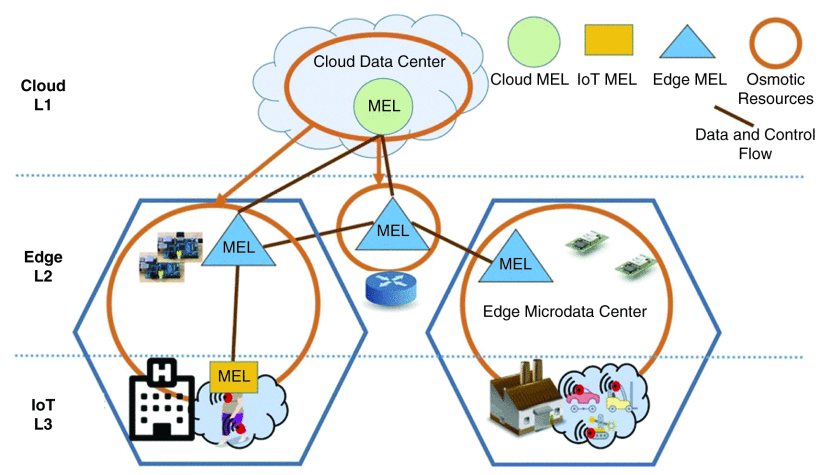
\includegraphics[width=0.8\linewidth]{figures/osmotic-architecture.png}
	\caption{Osmotic computing architecture reference. Picture taken from~\Cite{8781958}.}
	\label{fig:osmotic-computing}
\end{figure}

The purpose of an osmotic platform is to balance the needs of both the infrastructure and the applications by automatically relocating microservices
to appropriate deployment locations. This approach focuses mainly on systems that are centrally managed and coordinated.

\subsubsection{DR-BIP and DReAM framework}

The \emph{Dynamic Reconfigurable BIP} framework (DR-BIP)~\cite{10.1007/978-3-030-03424-5_20} includes three main aspects of dynamism: (I) the ability
to describe parametric system coordination for an arbitrary number of instances of component types, (II) the ability to add/delete components and
manage their interaction rules depending on dynamically changing conditions, and (III) allow services to seamlessly continue their activity on any
available device or computer (fluid architectures~\cite{taivalsaari2014liquid}).
The \emph{DR-BIP} framework is an extension of the \emph{Behavioral Interconnection Protocol} (BIP)~\cite{5719588} and
\emph{Dy-BIP} (a former extension that support dynamic interactions)~\cite{10.1007/978-3-642-30564-1_1}.

The DR-DIP framework provides support for runtime changes in the system, including component creation and removal, migration between motifs, and both
programmed and triggered reconfiguration.
The use of motifs allows components to interact with others based on their behavior and interaction rules within their new
motif, providing a flexible framework for coordination. The platform shares similarities with DReAM~\cite{de2020dream}, but the use of constraints
allows for more expressive coordination.

DR-BIP uses motifs as the basic unit for describing dynamic architectures (see~\Cref{fig:motif-concept}). Each motif includes the behavior of
components, the rules for interaction between components, and the rules for reconfiguring the motif, including adding, removing, or moving components.
Motifs are structurally organized as the deployment of component instances on a logical map.
Maps are arbitrary graph-like structures consisting of interconnected positions. Deployments relate components to positions on the map.
The definition of the motif is completed by two sets of rules: (I) the interaction rules, which define the behavior of the components and the
interaction between them, and (II) the reconfiguration rules, which define the conditions under which the motif can be reconfigured.

Systems are defined as collections of motif instances, each of which can evolve independently or in coordination with other motifs through shared
components or inter-motif reconfiguration rules. Inter-motif reconfiguration rules also allow for the creation and deletion of motif instances and
the exchange of components between motifs.

DR-BIP's behavior in a motif-based system is defined in a compositional way, where every motif has its own set of interactions determined by its
local structure. These interactions remain constant until the motif executes a reconfiguration action. In the absence of reconfigurations, the system
maintains a fixed architecture and operates like a normal BIP system. Interactions do not affect the architecture, while system and/or motif
reconfigurations change the architecture, but do not impact components, meaning running components retain their state, even though new components may
be added or removed.

\begin{figure}[ht]
	\centering
	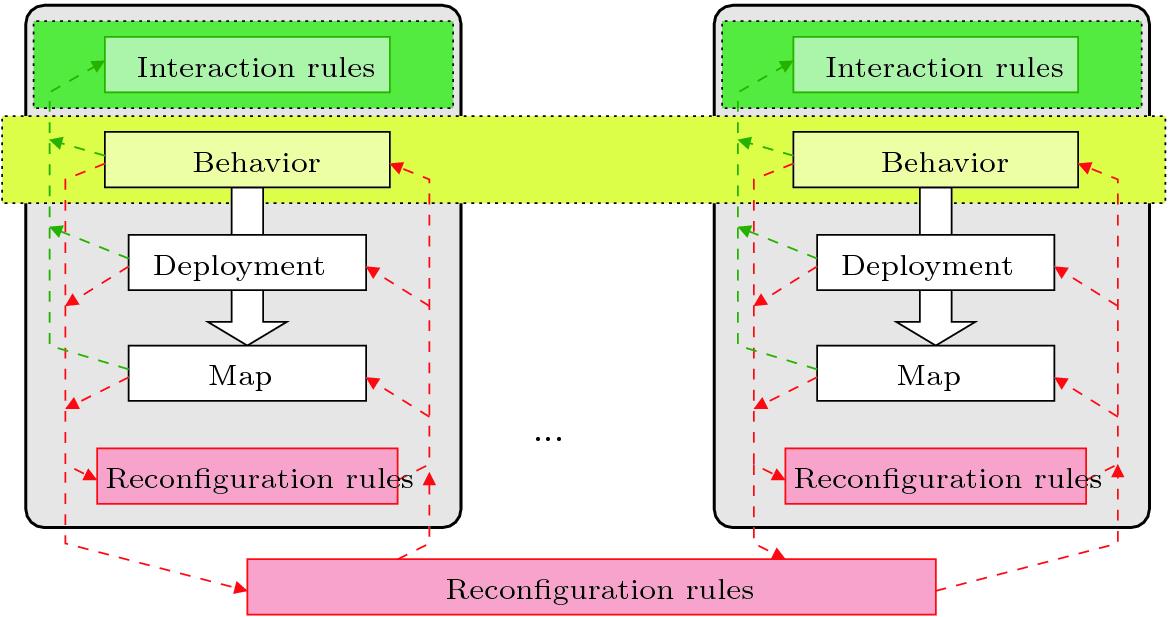
\includegraphics[width=0.8\linewidth]{figures/motif-concept.png}
	\caption{Motif-based System Concept. Picture taken from~\cite{10.1007/978-3-030-03424-5_20}.}
	\label{fig:motif-concept}
\end{figure}

% - New section ---------------------------------------------------------------

\section{Pulverization in Aggregate Computing and CPS}
\label{sec:pulverization-aggregate-computing-cps}

This section presents a brief overview of the state of the art in the field of aggregate computing and cyber-physical with a main focus on the
pulverization and which problems try to solve.

Self-organizing systems are a way of engineering distributed intelligence in which the system's global behavior and structure are achieved through
the continuous interaction of simple individual components. This approach allows for inherent adaptation to unexpected or unforeseeable situations
and has been applied in various contexts, such as human social behavior, and swarm robotics.

Artificial self-organizing systems are software-based systems that regulate their internal structures and behavior without external control, often by
mimicking the self-organization mechanisms observed in nature. Self-organizing approaches are applied to distributed cyber-physical systems (CPS),
where individual system components interact with each other based on physical proximity to collect and process information generated by distributed
sensors and use it to control the system behavior.

However, recent advances in technology have made modern CPS increasingly large-scale, heterogeneous, and dynamic, which makes it challenging to
engineer distributed intelligent systems that can be deployed in different contexts and exploit available resources opportunistically. To address
this problem, a framework based on the pulverization approach is proposed~\cite{fi12110203}, which breaks the overall system behavior into tiny
pieces of computation linked to sensors, actuators, and neighboring components. These sub-components can be deployed and wired separately, allowing
for a separation of concerns between the self-organization logic and the deployment context.

The pulverization approach can be implemented in the framework of Aggregate Computing~\cite{beal2015aggregate}, where global self-organizing behavior
can be specified declaratively by composing pure functions expressing increasingly complex distributed algorithms.
This approach allows for the design of distributed adaptive behavior for large-scale CPS that can be deployed in a deployment-independent way,
meaning that the behavioral description of the self-organization logic remains unchanged regardless of the specifics of the deployment context.

The pulverization approach was exercised simulating a CPS whose aim is to reduce the contribution of household winter heating to air pollution by
imposing a custom maximum temperature relative to the level of particulate matter (PM) in the area surrounding the household~\cite{fi12110203}.
The system implements the functionality in a self-organization fashion, where there isn't a central coordinator and the system autonomously organizes
its behaviour even in the face of disturbance.
The goal of the experiment is to show that via the pulverization approach, the system's business logic, defined once, can be reused in different
deployment schemes, preserving its functional behavior.

Another initial research effort~\cite{9599177} was made by combining the pulverization approach with the multi-tier programming
paradigm~\cite{weisenburger2020survey}.
The multi-tier programming paradigm defines a distributed architecture in a single compilation unit with a single language. Once the program is
specified, the compiler (or the runtime) is responsible for splitting the computation among different peers.
A language that supports multi-tier programming is \emph{ScalaLoci}~\cite{weisenburger2018distributed, weisenburger2020implementing}, a type-safe
multi-tier language hosted in Scala.
A ScalaLoci application is structured through \emph{peers} and \emph{ties,}where peers abstract over the locations representing the components of an
application, while the ties define the connection between peers. Only tied peers can communicate with each other.
The example provided in~\cite{9599177} shows how the pulverization approach can be fitted into the multi-tier programming paradigm, by defining
a logical node as a peer which in turn is composed of a set of peers representing the pulverized device.
Moreover, the example shows the conjunction of ScaFi, a Scala internal DSL that can run on the JVM or in the browser and ScalaLoci showing
how this could be the foundation stone of a unified framework living in the Scala ecosystem.
Finally, the example shows how different deployment schemes can be defined by changing the ties between peers by preserving the functional behaviour
of the system.

%----------------------------------------------------------------------------------------

% Requirements --------------------------------------------------------------------------
\chapter{Requirements}
\label{chap:requirements}

This chapter introduces the pulverization approach by explaining the terminologies and concepts that will be used in the rest of the thesis.
The logic that governs pulverization will be discussed by going on to give some examples of pulverized systems.
Next, the requirements that the framework must have to implement and concretize the pulverization concepts are reported. Finally, the
chapter concludes by reporting some relevant scenarios in which it makes sense to test the effectiveness of the framework.

\section{Pulverization domain model}
\label{sec:pulverization-domain-model}

Pulverization is an approach to conceive self-organization in distributed systems that facilitate deployment independence, i.e., the ability of an
application to run with no change on various deployments while retaining its original functional semantics.
The main idea is to organize the structure and the behaviour of a system in a way that the developer can focus on the logical model, abstracting from
the deployment details, scheduling and communication.
The logical model can be partitioned into a set of software components that can be deployed on the available infrastructure, while the application
logic will preserve the functional goals independently from the actual deployment.

To better formalize the terminology coming from the pulverization, the following ubiquitous language is proposed in~\Cref{tab:ubiquitous-language}.

\begin{table}
	\begin{tabularx}{\textwidth}{l X}
		\toprule
		\textbf{Concept}          & \textbf{Definition}                                                                                             \\
		\midrule
		Sensors                   & Component that represents a set of logical \emph{sensors}                                                       \\
		Actuators                 & Component that represents a set of logical \emph{actuators}                                                     \\
		Behaviour                 & Component that models the device behaviour                                                                      \\
		Communication             & Component that handles the interaction with neighbours (other devices)                                          \\
		State                     & Component the holds the representation of the device's knowledge                                                \\
		Thin host                 & A device that has limited computational power and memory                                                        \\
		Thick host                & A device that has a powerful computational power and memory                                                     \\
		Logical device            & A logical representation of a device composed of several components which they can be deployed on the available
		infrastructure                                                                                                                              \\
		Logical neighbouring link & Defines a logical connection between two logical devices defining the network topology.
		The aforementioned structure can change over time.                                                                                          \\
		\bottomrule
	\end{tabularx}
	\label{tab:ubiquitous-language}
	\caption{Pulverization Ubiquitous language.}
\end{table}

\begin{figure}
	\centering
	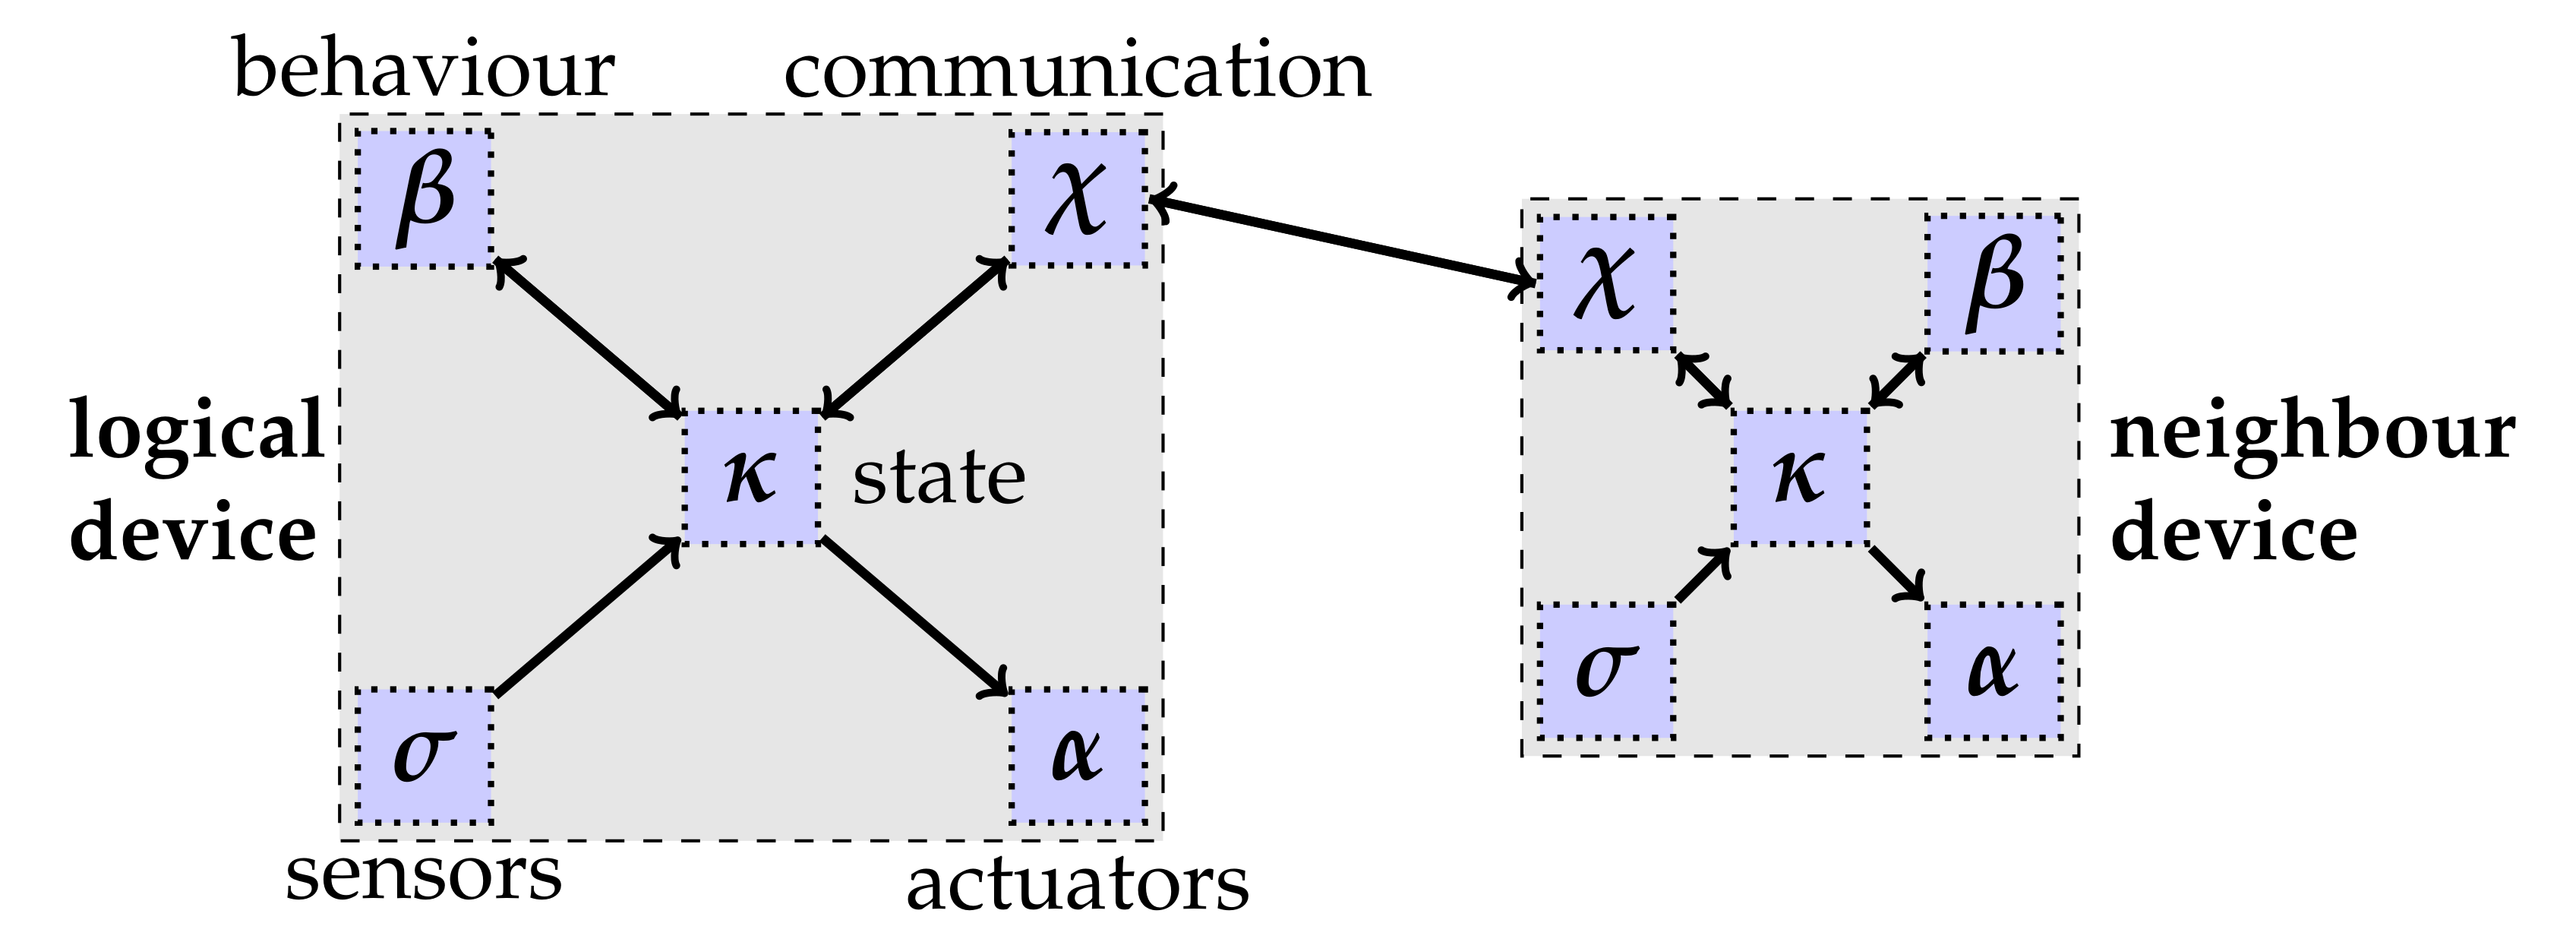
\includegraphics[width=\textwidth]{figures/original-components-interactions.png}
	\caption{Representation of a logical device split into its components and a connection with one of its neighbours}
	\label{fig:logical-device}
\end{figure}

Henceforth, concepts characterizing pulverization will be used with the meaning given in~\Cref{tab:ubiquitous-language}.

A \emph{Logical Device} is the representation of a device in the system abstracting from the specific deployment details.
It is composed of \emph{five} components: \emph{Sensors}, \emph{Actuators}, \emph{Behaviour}, \emph{Communication} and \emph{State} while the
interaction between them determines the device's logic in the system. The~\Cref{fig:logical-device} shows a representation of a logical device
split into its components defining also a link with another device.

The \emph{Sensors} $\sigma$ and \emph{Actuators} $\alpha$ components represent the way the device interacts with the environment: the former is used
to acquire information from the environment, while the latter is used to actuate on the environment.
The \emph{State} $\kappa$ component represents the device's knowledge and abstract from the actual storage mechanism or representation.
The \emph{Communication} $\chi$ component handles the interaction with neighbours by holding the information about the identity of the neighbours and
how to reach them. The send and receive operations occur through respectively the \emph{input channels} and the \emph{output channels}, where the
output channel of a device is connected to the input channel of its neighbours.
Finally, the \emph{Behaviour} $\beta$ component models the device behaviour via a \emph{function} which maps the state of the device to a new state,
defines a set of prescriptive actions to be performed and a set of coordination data to be propagated to the neighbours.

Each device performs a MAPE-like cycle that includes the following steps and that defines the interactions between the device's subcomponents as
depicted in~\Cref{fig:logical-device}, where the arrows denote the message flow:

\begin{enumerate}
	\item \textbf{Context acquisition:} the device acquires information from its sensors and communications, storing them in the device state
	\item \textbf{Computation:} the device behaviour function is computed against the device state
	\item \textbf{Coordination data propagation:} coordination data is set to all the device neighbours
	\item \textbf{Actuation:} the actuators are activated to execute a set of prescriptive actions
\end{enumerate}

A platform is a collection of physical \emph{hosts} connected by a dynamic graph of physical network links, representing the communication channel
between two hosts. A host is an entity with a unique identifier (e.g. an IP address, URI resource, etc.) and can be a computer system, an embedded
device holding sensors and actuators, a virtual machine or a software container. The type of communication channel (the link between hosts) may
vary depending on the underlying network infrastructure and protocols.
The \emph{hosts} types are divided into two categories: \emph{thin hosts} and \emph{thick hosts}. Thin hosts are devices with limited computational
power and memory, while thick hosts can compute and may even do so on behalf of multiple logical devices.

\begin{figure}
	\centering
	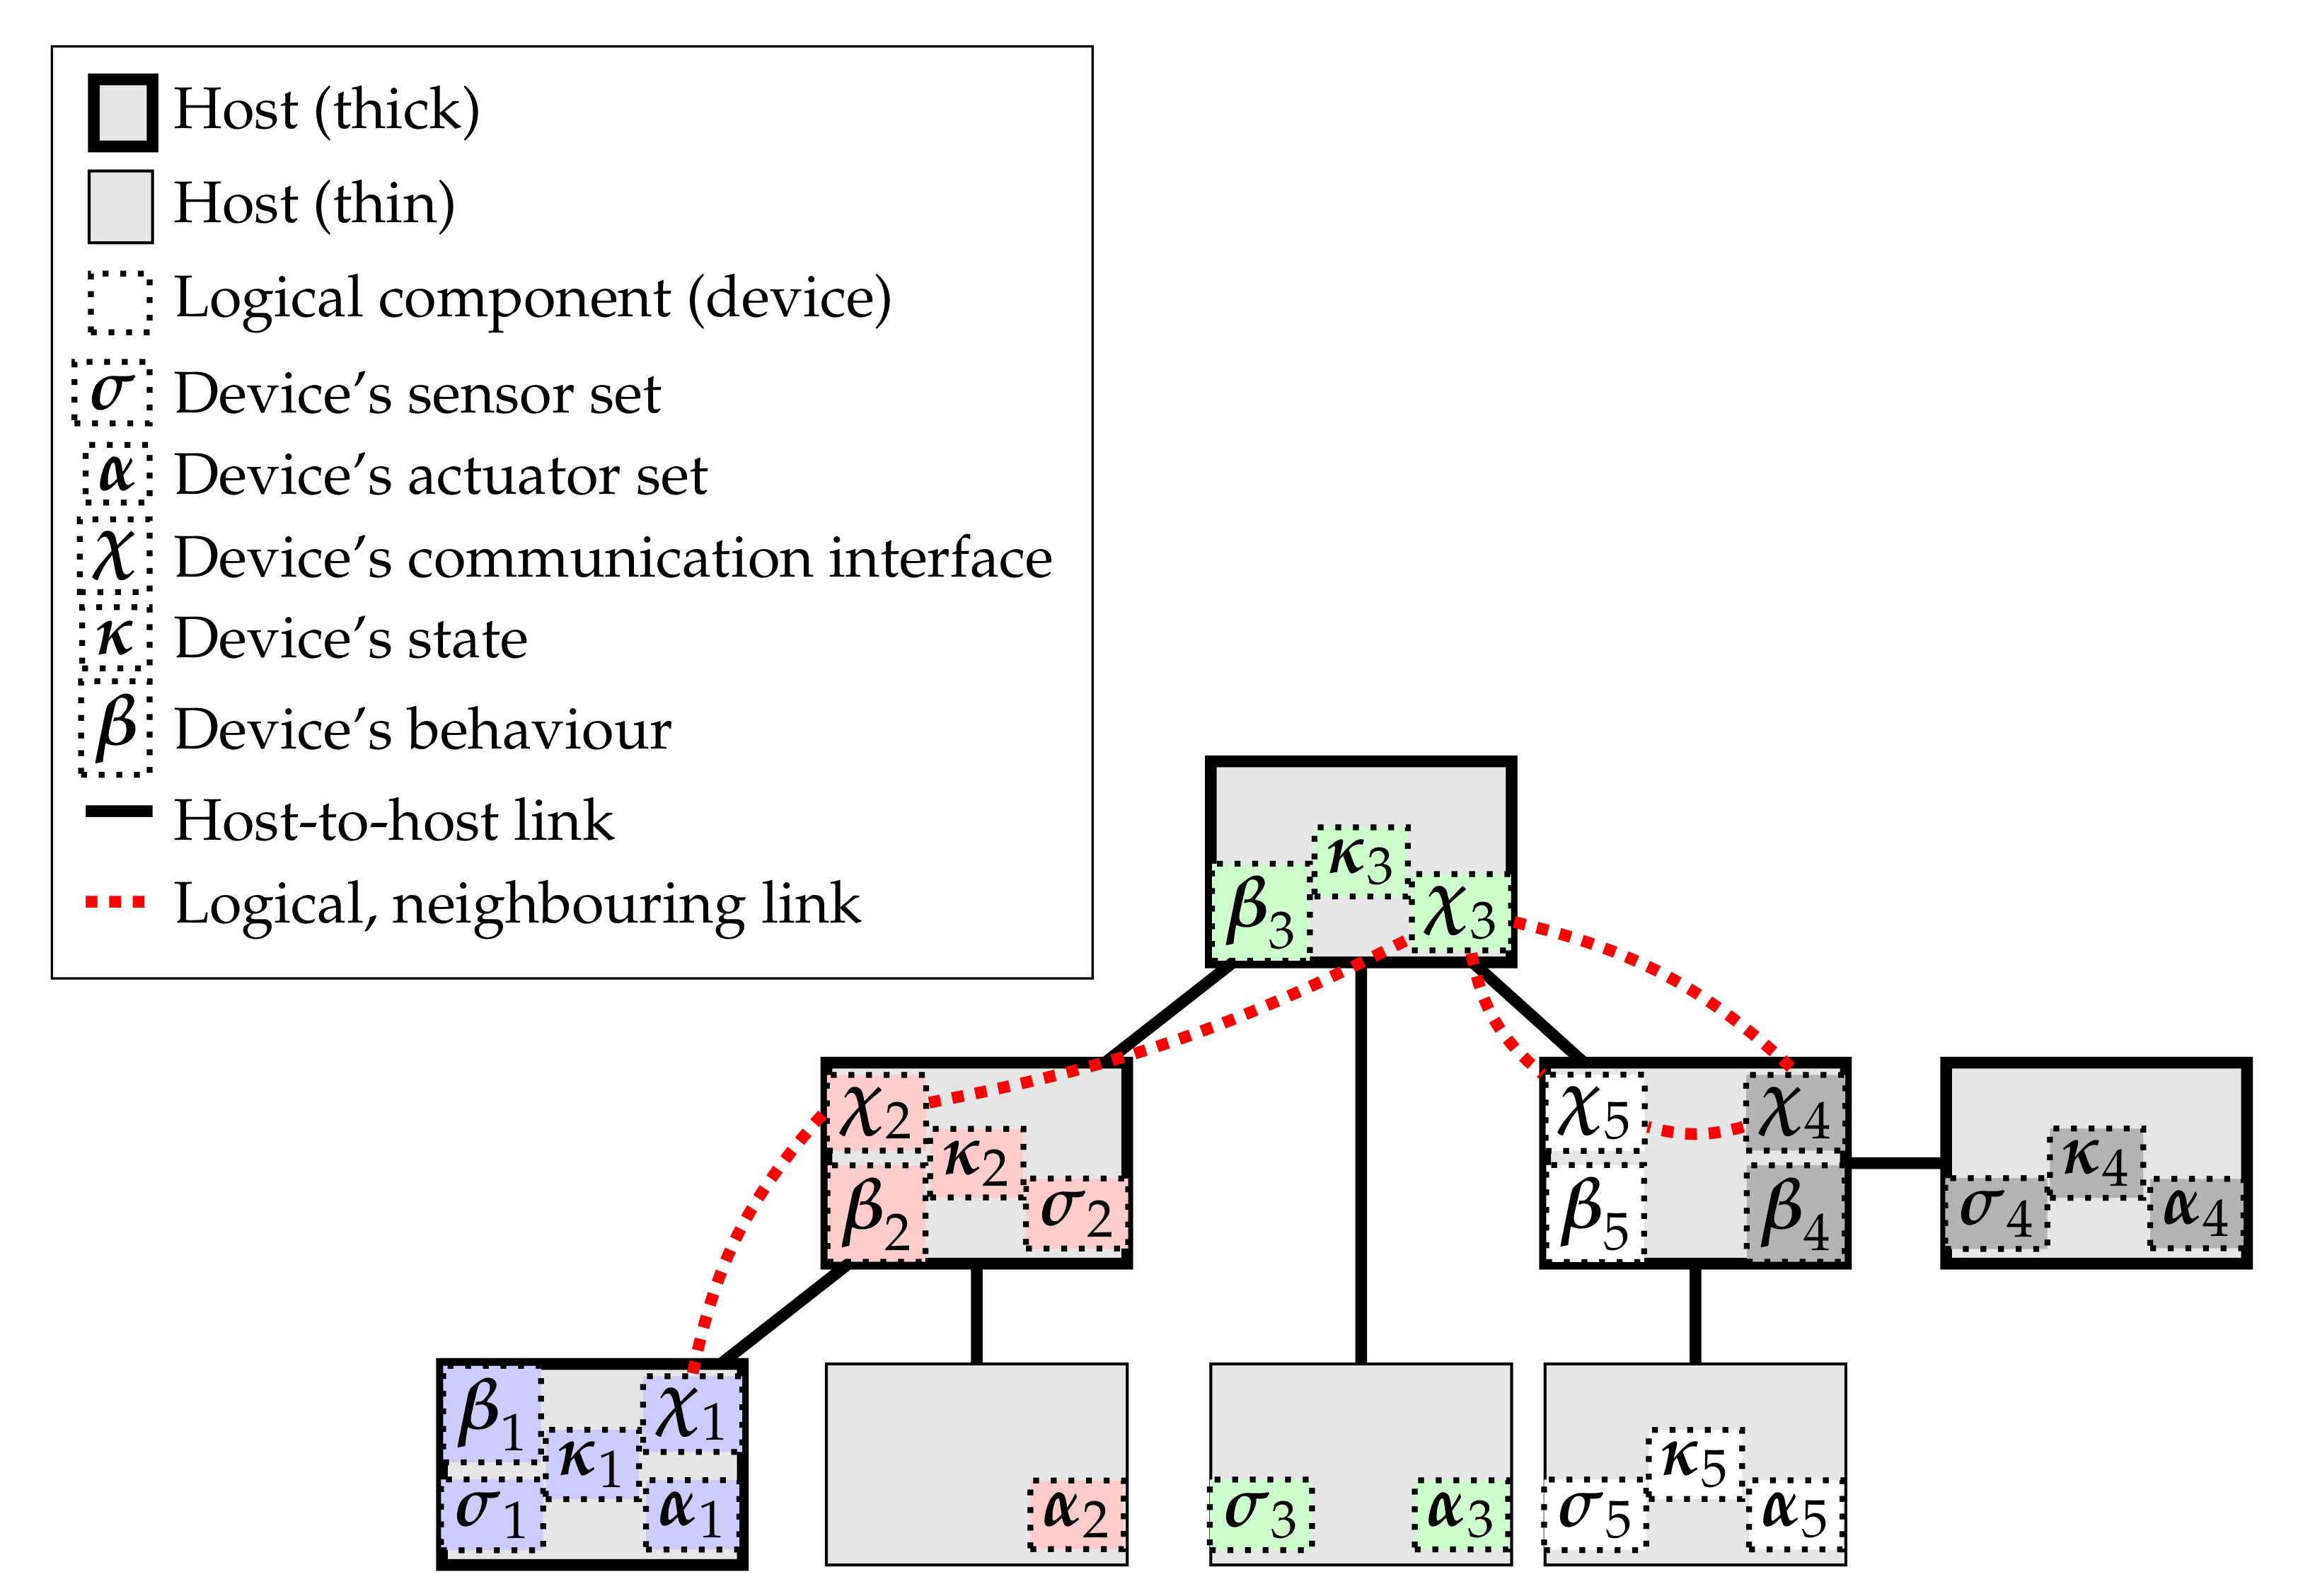
\includegraphics[width=0.7\linewidth]{figures/cps-example.png}
	\caption{Example of instantiation of the CPS model.}
	\label{fig:cps-example}
\end{figure}

\begin{figure}
	\centering
	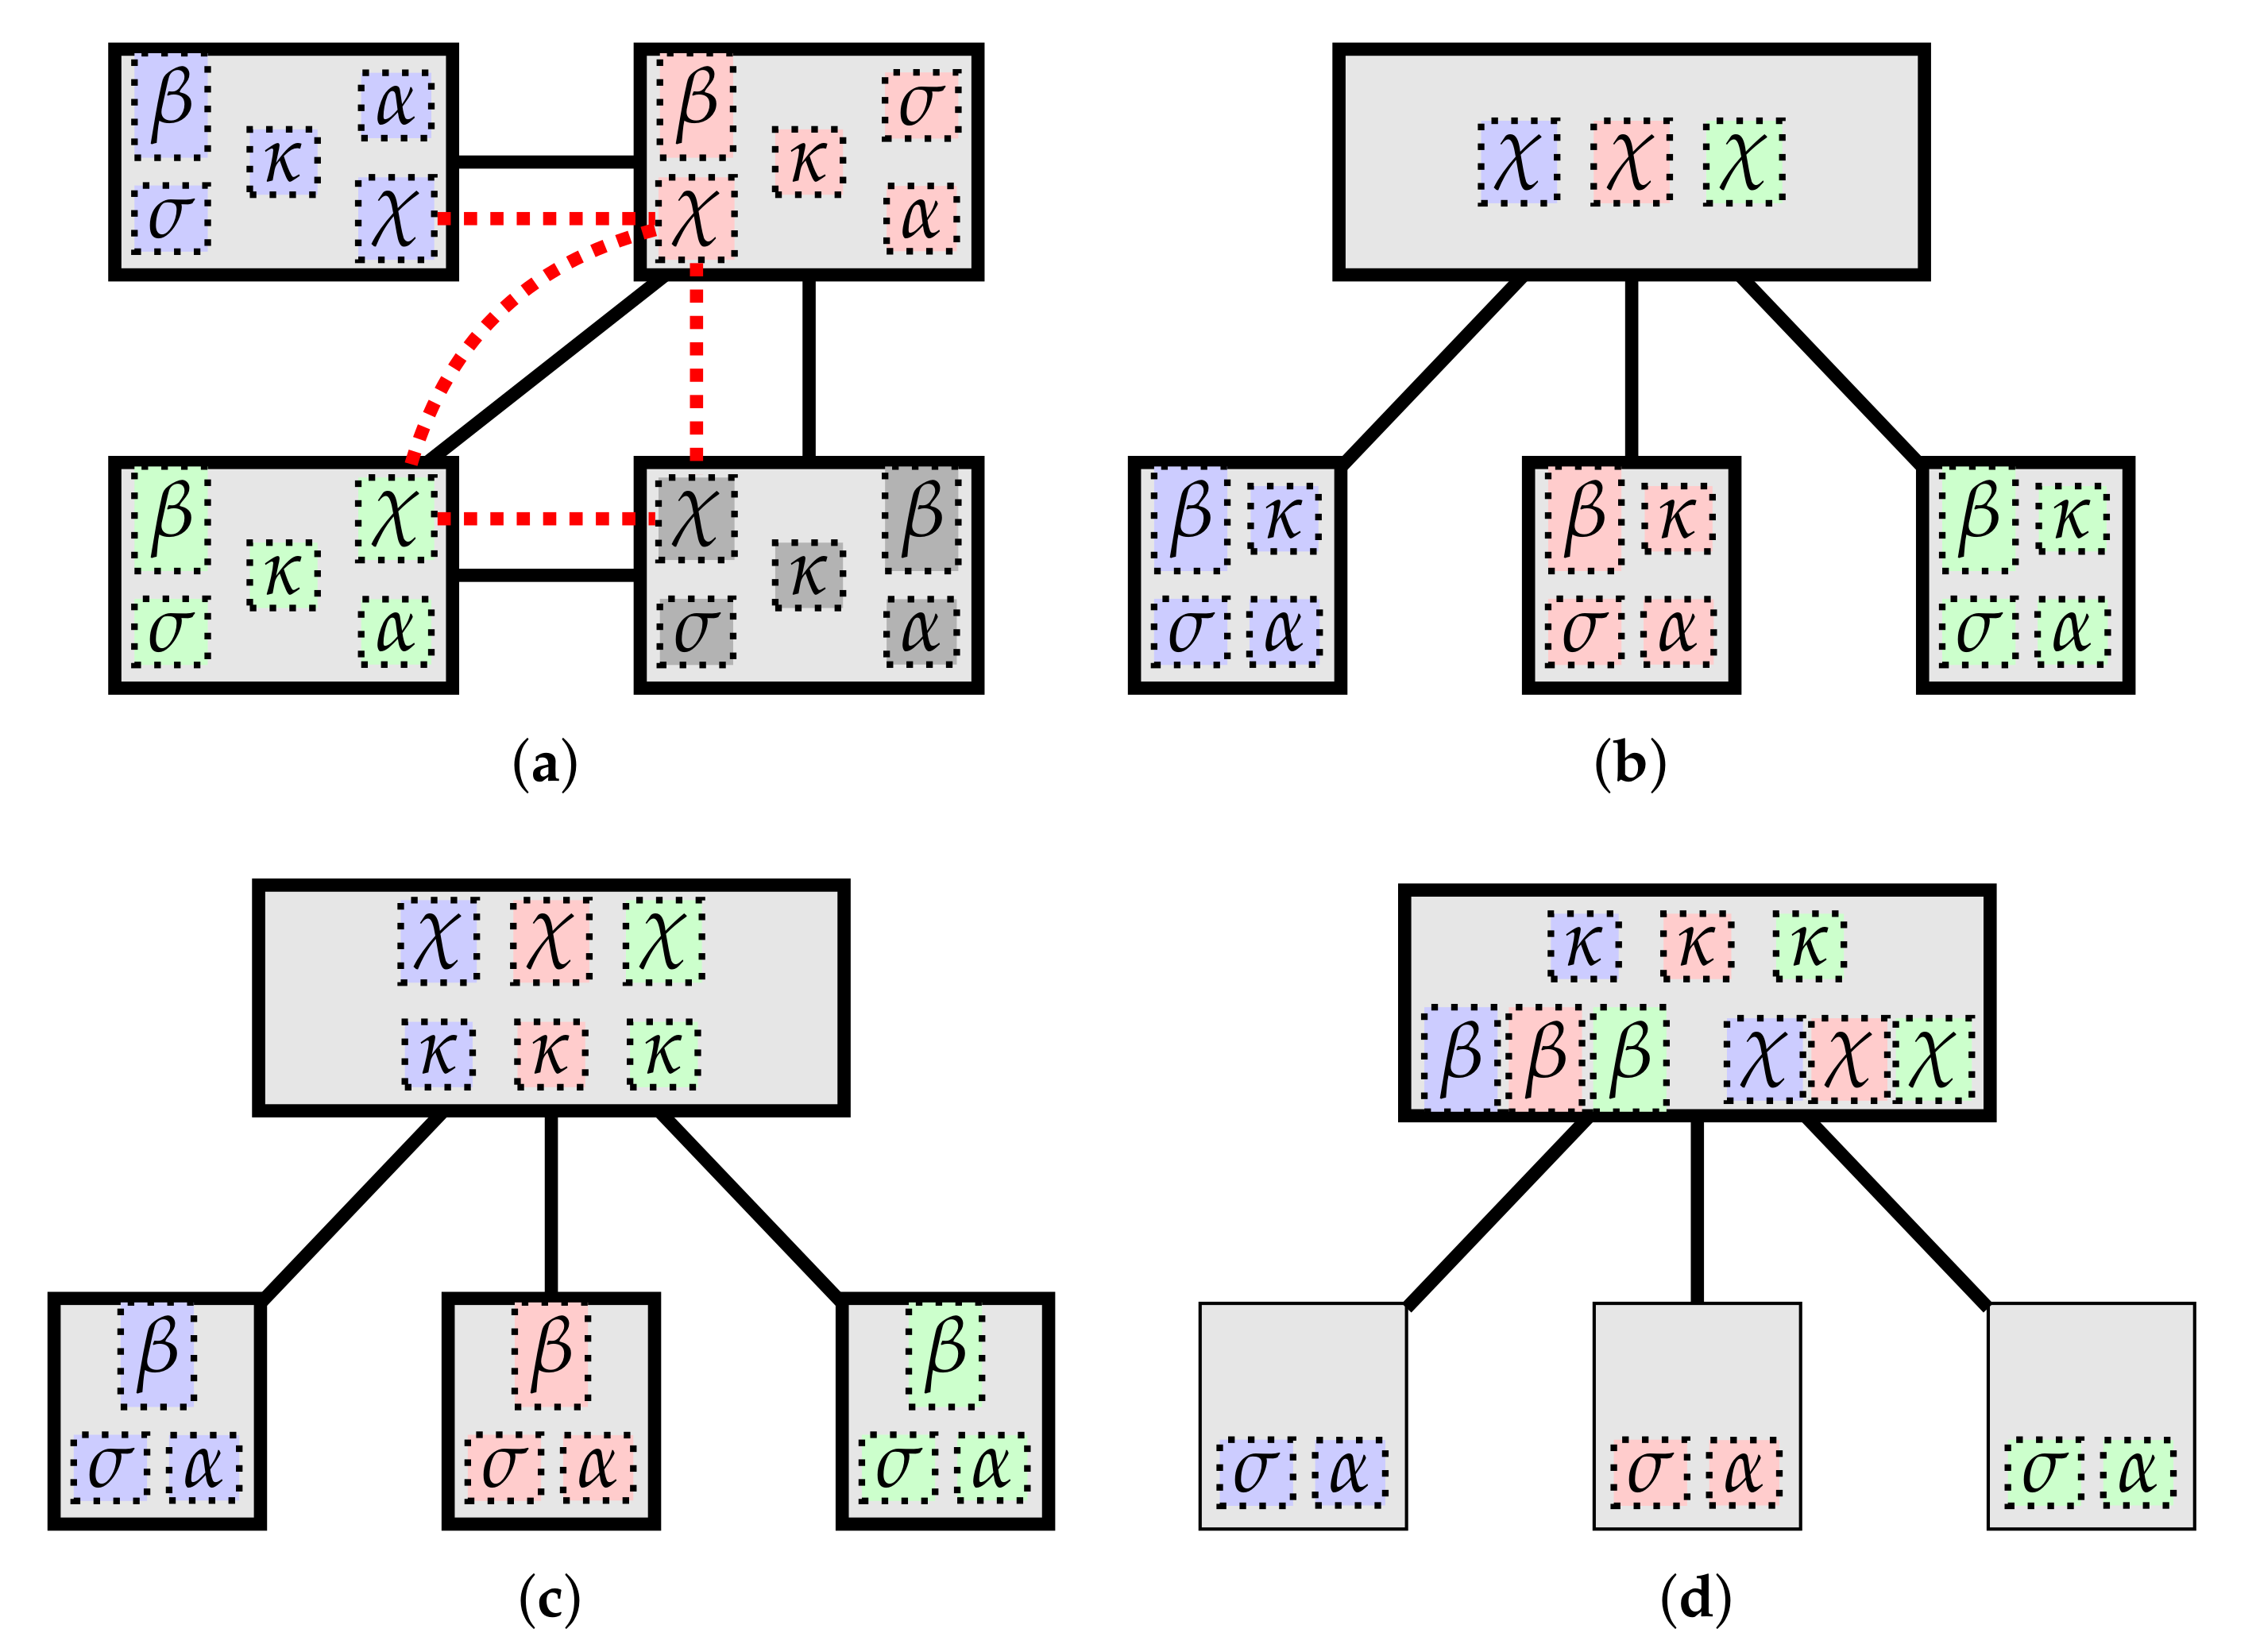
\includegraphics[width=0.7\linewidth]{figures/notable-deployments.png}
	\caption{\textbf{(a)} Peer-to-peer style; \textbf{(b)} broker-based style (e.g. MQTT); \textbf{(c)} Big data in the cloud style; \textbf{(d)} embedded device with sensors/actuators.}
	\label{fig:notable-deployments}
\end{figure}

The deployment of the CPS can be defined as an \emph{allocation map} placing each component of each device to specific hosts in the platform.
An example of a deployment can be seen in~\Cref{fig:cps-example}. In the example is assumed that all the sensors and actuators are deployed on the
same host, though this is not a requirement, sensors and actuators may be deployed on different hosts.

Examples of deployment are provided in~\Cref{fig:notable-deployments} showing an increasing number of responsibilities are centralized.
The~\Cref{fig:notable-deployments}a shows a peer-to-peer style deployment where, for each device, all the components are deployed on the same host.
This style is not suitable in a sensor network where a device is designed to operate for a long time using solely battery power and is not equipped
with enough power to host a $\beta$-component.
The~\Cref{fig:notable-deployments}b shows a broker-based style deployment where all the $\chi$-components are deployed on a separate host (broker).
This is a common scenario in IoT systems where a broker is used to handle the communication between devices.
The~\Cref{fig:notable-deployments}c shows big data in the cloud style deployment where all the $\kappa$-components are deployed in the cloud
enabling big-data analysis.
The~\Cref{fig:notable-deployments}d shows an embedded device with sensors/actuators style deployment where all the $\alpha$ and $\sigma$-components
are deployed on the same thin host while all the remaining components are deployed on a thick host. This scenario covers the case of a device
with limited computational power and memory by offloading the $\beta$-component to a thick host.

% - New section ---------------------------------------------------------------

\section{Framework requirements}
\label{sec:framework-requirements}

The main objective of this thesis work is to develop a framework that can ``fill the gap'' between the modelling of a CPS (and its simulation) and
the physical deployment of the system on an infrastructure.
The framework should model the pulverization concept and provide a clear separation between the behaviour of the overall system and low-level
details of the deployment via a simple and concise API.
Also, the framework must capture the concepts defined by the pulverizing approach so that it has a good foundation on which the framework can
evolve.

\subsubsection{Business requirements}
\label{sec:business-requirements}

As previously mentioned, the main objective of the framework is to provide a way to deploy CPSs via the pulverization approach.
The business requirements identified are reported as follows:

\begin{itemize}
	\item The pulverization approach can be used to simply and effectively deploy a system
	\item The framework should be flexible to support different deployment strategies
	\item The framework should be extensible to support different communication protocols
\end{itemize}

\subsubsection{User requirements}
\label{sec:user-requirements}

The user requirements are the requirements that are identified from the perspective of the developer who will use the framework.
The user requirements identified are reported as follows:

\begin{itemize}
	\item It should be possible to configure the system to deploy by defining the structure of each device \emph{logical device}
	\item It should be possible to configure the \emph{deployment unit} for each \emph{logical device}
	\item It should be possible to configure the \emph{logical devices} and \emph{deployment unit} via a DSL
	\item The \emph{sensors} component should be created
	\item The \emph{actuators} component should be created
	\item The \emph{communication} component should be created
	\item The \emph{behaviour} component should be created
	\item The \emph{state} component should be created
\end{itemize}

\subsubsection{Functional requirements}
\label{sec:functional-requirements}

The functional requirements, obtained from the user requirements, are reported below:

\begin{itemize}
	\item Multiple \emph{logical devices} can be defined
	\item For each \emph{logical device}, the \emph{components} that compose it can be defined
	\item Each \emph{component} defined for a \emph{logical device} must be configured to be deployed on a specific tier of the infrastructure
	\item A check must be performed to ensure that the configuration of the \emph{logical devices} is valid and consistent
	\item Links between \emph{logical devices} can be defined
	\item Multiple deployment units can be defined for each \emph{logical device} using the system configuration
	\item The user-defined \emph{components} can be added to the deployment unit
	\item The \emph{deployment unit} can be started
	\item The \emph{deployment unit} can be stopped
	\item Prevent the run of the \emph{deployment unit} if the configuration is not honored
	\item Different protocols can be added to the \emph{deployment unit} to enable intra-component communication
	\item For each component, a custom implementation of the logic that implements how the communication with other components should occur can be
	      provided
\end{itemize}

\subsubsection{Non-functional requirements}
\label{sec:non-functional-requirements}

\begin{itemize}
	\item The framework should be easy to use by providing a simple and clean API simplifying the development of the system and adoption of the
	      framework
	\item The framework should be extensible in the sense that the user can customize some aspects of the framework like the communication protocols,
	      and the logic of each component
	\item The framework should be flexible to support different deployment strategies coping with different scenarios and infrastructures
	\item The framework should support a wide range of architectures to support a heterogeneous set of devices enabling wide adoption of the
	      framework
\end{itemize}


% - New section ---------------------------------------------------------------

\section{Reference scenarios}
\label{sec:reference-scenarios}

%----------------------------------------------------------------------------------------

% Design --------------------------------------------------------------------------------
\chapter{Design} % possible chapter for Projects
\label{chap:design}

This chapter describes the design choices and the overall architecture of the framework. \todo{Expand the introduction}

\section{Framework architecture}
\label{sec:arch-design}

The framework is articulated in modules: each module takes into account a specific aspect of the pulverization.
The modularity of the framework enables from one side, the possibility to use only the needed modules, preventing the bloating of the project;
on the other side, modularity allows the customization of some implementations of the framework.

The two fundamentals modules of the pulverization framework are: \emph{core} and \emph{platform} which respectively define the core concepts
of pulverization like the type of components and all the logic needed to run the pulverized system like defining the components reference,
loading the user-defined components and setup the communications between all of them.

The third module is \emph{rabbitmq-platform} which is highly dependent on the two modules described above and its purpose is to rely on
\textbf{RabbitMQ}\footnote{\textbf{RabbitMQ} is an open-source message-broker (or message-oriented-middleware) that originally implement
	the \emph{AMQP} protocol and has since been extended with a plug-in architecture to support other protocols like \emph{MQTT}.} to enable
the communications between all the components.
This component manages all the low-level aspects related to communication like the connection to the broker, declaring queues and so on.

In~\Cref{fig:package-diagram} are represented all the framework's modules and the relationship between them.

\begin{figure}
	\centering
	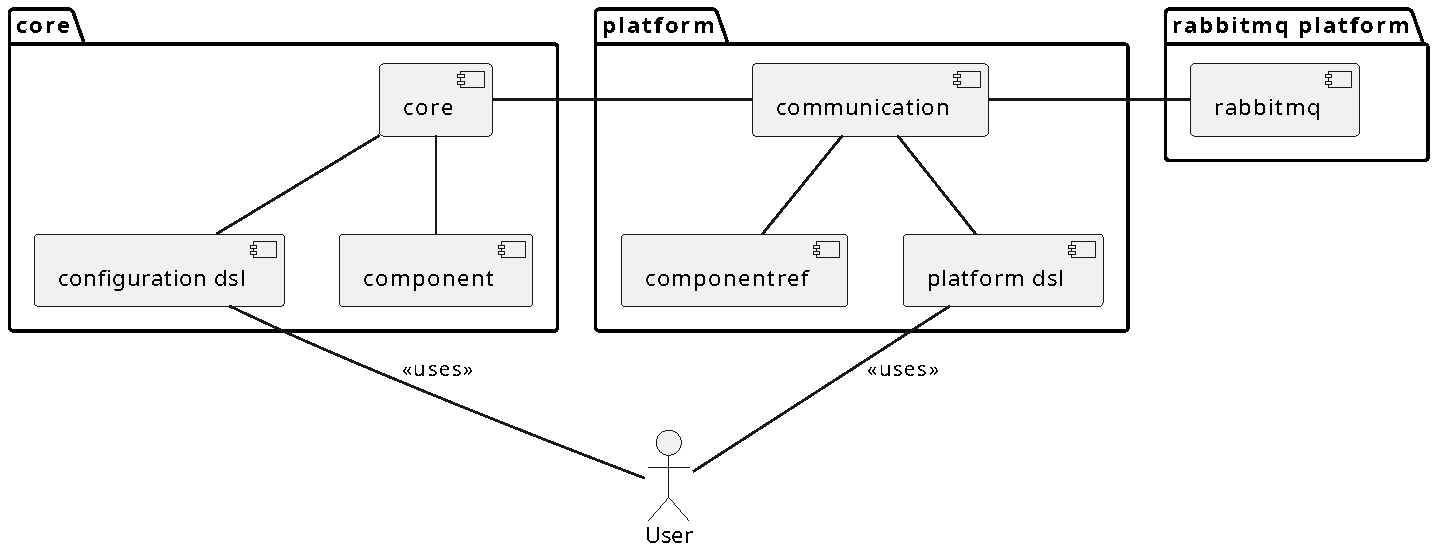
\includegraphics[width=\textwidth]{figures/package-diagram.pdf}
	\caption{Package diagram showing the modules that constitute the framework and their relationship.}
	\label{fig:package-diagram}
\end{figure}

In the~\Cref{tab:framework-modules} are reported a synthetic representation of the modules that constitute the framework with a corresponding
description.

\begin{table}
	\begin{tabularx}{\textwidth}{l X}
		\toprule
		\textbf{Module}            & \textbf{Description}                                                                                             \\ \midrule
		\texttt{Core}              & Defines all the pulverization concepts, exposing them as interfaces.
		Provides a DSL to specify the device types.                                                                                                   \\
		\texttt{Platform}          & Is responsible for executing all the device's components on the available infrastructure.
		Provides a DSL to configure the platform specifying which components should be used.                                                          \\
		\texttt{RabbitMQ Platform} & Represents a possible implementation for enabling intra-component communication leveraging RabbitMQ as protocol. \\ \bottomrule
	\end{tabularx}
	\caption{A tabular representation of the modules that constitute the framework.}
	\label{tab:framework-modules}
\end{table}

The pulverization framework relies on a three-level architecture. Each level of the framework's architecture is designed to use the functionalities
of the layer above and makes accessible their functionalities to the layer below.

The described architecture takes with it the implicit ``one-way dependency'' where the layer below depends on the layer above and not vice versa.
The~\Cref{fig:framework-architecture} depicts the architecture's choice made to design and build the framework.

\begin{figure}
	\centering
	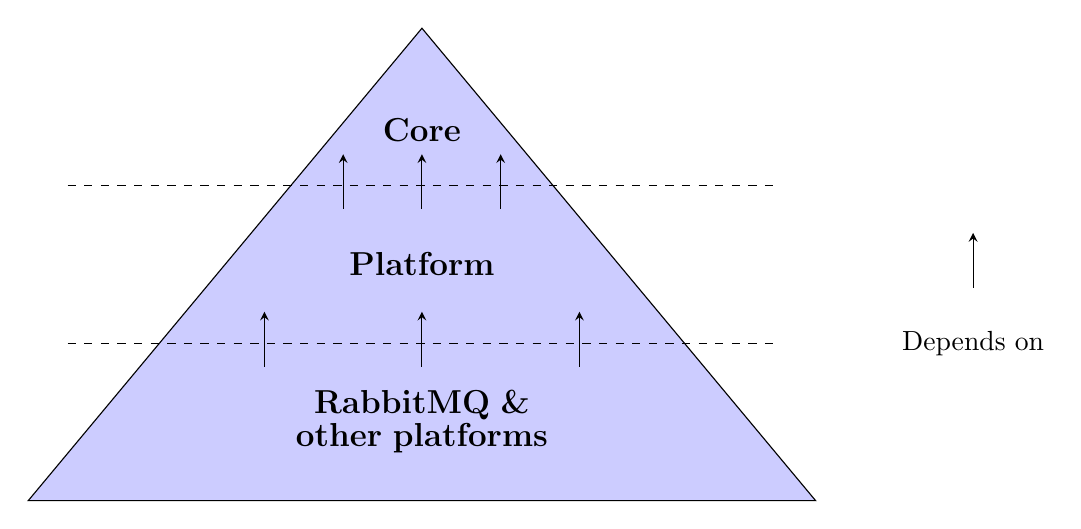
\begin{tikzpicture}
		\tikzstyle{fontbf} = [rectangle,text width=5cm,text centered,font=\bfseries]
		\draw[fill=blue!20] (0,0) -- (-5, -6) -- (5, -6) -- cycle;
		\draw[dashed] (-4.5,-2) -- (4.5,-2);
		\draw[dashed] (-4.5,-4) -- (4.5,-4);
		\draw[stealth-](0,-1.6) -- (0,-2.3);
		\draw[stealth-](-1,-1.6) -- (-1,-2.3);
		\draw[stealth-](1,-1.6) -- (1,-2.3);

		\draw[stealth-](0,-3.6) -- (0,-4.3);
		\draw[stealth-](-2,-3.6) -- (-2,-4.3);
		\draw[stealth-](2,-3.6) -- (2,-4.3);

		\draw[stealth-](7,-2.6) -- (7,-3.3);
		\node at (7,-4) {Depends on};

		\node[fontbf] at (0, -1.3) {\large Core};
		\node[fontbf] at (0, -3) {\large Platform};
		\node[fontbf] at (0, -5) {\large RabbitMQ \& other platforms};
	\end{tikzpicture}
	\caption{Architectural diagram showing how the pulverization framework is designed.}
	\label{fig:framework-architecture}
\end{figure}

Since this is a framework, it will likely be used by several users; therefore, it is strategic to minimize the cognitive effort that the user will
have to make to use it.

For a framework to be successful and usable, it must be able to provide an incremental approach to its use,
meaning that it must provide only the abstractions necessary for its use while at the same time providing clarity in its innermost components so that
the user can understand how it works and possibly extend the framework with external modules.

The ``pyramid architecture'' used by the framework tries to apply the concept described above (\Cref{fig:pyramid-user-knowledge}):
the tip of the pyramid represents the components' abstraction defined by the pulverization and those components are used and built by the user.
Those abstraction needs to be as clear as possible from a software engineering perspective.
As you move down the pyramid, the complexity of the modules increases but the user's knowledge of them decreases.

\begin{figure}
	\centering
	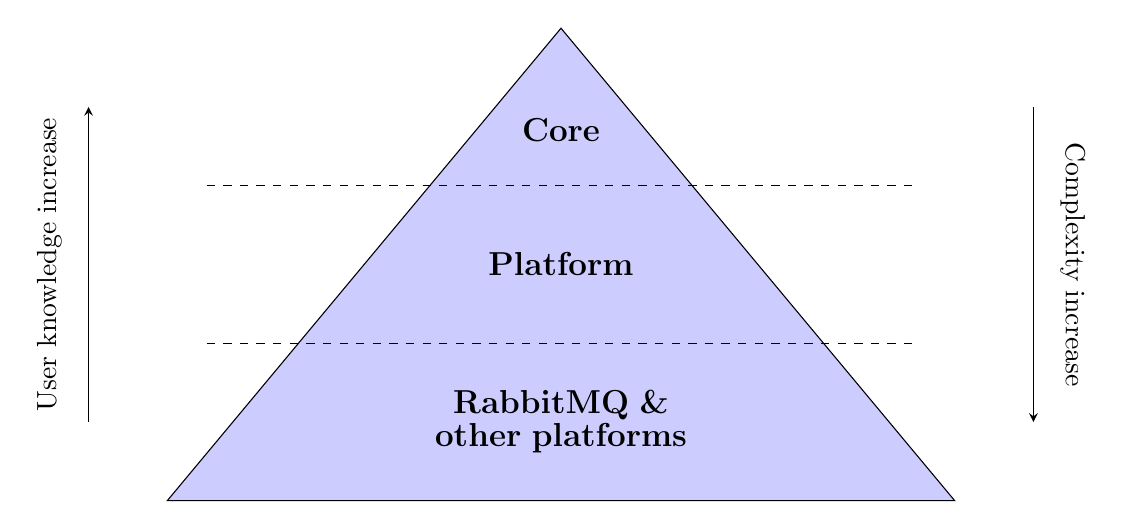
\begin{tikzpicture}
		\tikzstyle{fontbf} = [rectangle,text width=5cm,text centered,font=\bfseries]
		\draw[fill=blue!20] (0,0) -- (-5, -6) -- (5, -6) -- cycle;
		\draw[dashed] (-4.5,-2) -- (4.5,-2);
		\draw[dashed] (-4.5,-4) -- (4.5,-4);
		\draw [-stealth](6,-1) -- (6,-5);
		\draw [stealth-](-6,-1) -- (-6,-5);
		\node[rotate=-90] at (6.5,-3) {Complexity increase};
		\node[rotate=90] at (-6.5,-3) {User knowledge increase};
		\node[fontbf] at (0, -1.3) {\large Core};
		\node[fontbf] at (0, -3) {\large Platform};
		\node[fontbf] at (0, -5) {\large RabbitMQ \& other platforms};
	\end{tikzpicture}
	\caption{A correlation between the framework's complexity and the required user's knowledge to use the framework.}
	\label{fig:pyramid-user-knowledge}
\end{figure}

By designing the framework in this way, we open up different usage scenarios such as a basic use that requires only an understanding of the
basic concepts, to advanced uses that require a deep understanding of the framework enabling its complete usage and extension.

\todo{valutare se espandere qui con esempi o altro}

The sections below will describe the architectural choices made for each framework's module.

\subsection{Core module}
\label{sec:core-module}

Architecturally, the \emph{core} module is rather simple. Its simplicity is a consequence of the fact that this module is the main entry point
for the user, and the lower the complexity of this module, the faster the user can become familiar with the framework.
Moreover, a correct design of the interfaces defined in the \emph{core} module is a crucial aspect to consider to be aligned with the
pulverization concepts illustrated in the article~\cite{fi12110203}.

The pulverization represents a device as the combination of five components: \textbf{state}, \textbf{behaviour}, \textbf{communication},
\textbf{sensors} and \textbf{actuators}~\cite{fi12110203}.
All of those concepts are modeled by the framework through interfaces that the user will implement based on the specific scenario.

\begin{figure}
	\centering
	\missingfigure[figwidth=\textwidth]{Create a class diagram showing the interfaces defined by the core module}
	\caption{Class diagram showing the interfaces defined by the core module.}
	\label{fig:core-module-architecture}
\end{figure}

The~\Cref{fig:core-module-architecture} shows the concepts defined by the core module and their relationship.

This module provides a DSL to generate the configuration needed for the platform to run. In particular, the DSL provides a simple, clean and handy
way to create in a declarative fashion how many logical devices should the platform manage, and how those devices are made.

\subsection{Platform module}
\label{sec:platform-module}

The platform module defines the enabling concepts for system execution like intra-component communication and provides an abstraction for
representing a remote component and how to reach it; finally, it manages all the machinery needed to run the system.

The highly distributed nature of the pulverization has forced the design phase to abstract from the actual place where components are actually
deployed; in this way, we avoid the need for the user to specify and/or manage specific aspects of deployment but can focus solely on
application logic while remaining adherent to the objectives of the pulverization, which among many want to separate aspects of
deployment from aspects of application logic~\cite{fi12110203}.

Although the abstractions defined in this module are fundamental to the execution of the system, their understanding by the user is not essential.
Nevertheless, their understanding becomes crucial when the user wants to extend the framework with new features, like implementing a new protocol to
enable intra-communication components.

As said before, communication between components is a fundamental aspect to consider; for this reason, the \emph{communicator} concept comes in.
The communicator abstracts the way how the communication between two (pulverized) components occurs, defining how two components communicate with
each other. The design of this component abstracts from the message format and the type of the involved components, effectively making the
communicator highly generic and delegating all those complexities to the platform.

Finally, the platform module provides a DSL to allow the user to instantiate the platform and then actually run the system.
The DSL allows, declaratively, to specify the components intended to be executed in that specific deployment unit, as well as indicate which
specific communicator implementation to use. In~\Cref{fig:platform-module-architecture} is depicted the overall architecture of the platform module.

\begin{figure}
	\centering
	\missingfigure[figwidth=\textwidth]{Create a class diagram showing the interfaces defined by the platform module}
	\caption{Class diagram showing the interfaces defined by the platform module.}
	\label{fig:platform-module-architecture}
\end{figure}

\subsection{Rabbitmq-platform module}
\label{sec:rabbitmq-platform-module}

This module implements a possible communicator that bases its operation on RabbitMQ. Although this module, at the time of writing, represents
the only implementation of a communicator, this does not mean that it should be the only possible solution.
Other communicators based on different technologies and infrastructures will likely be implemented in the future.

In this module, all the communication aspects that will be used for communication between components of the pulverized system are defined.
The design of the framework delegates to these types of implementations to handle low-level aspects like connections, retry on failure and so on.

While this module (or this kind of module more generally) requires a very good understanding of the concepts defined in
section~\ref{sec:platform-module} to be implemented, it requires no cognitive effort on the part of the user to be used.
\todo{Forward reference alla sezione dove si spiegano i dettagli implementativi di questo modulo}

% - New section ---------------------------------------------------------------

\section{Data flow in the framework}
\label{sec:framework-data-flow}

Pulverization based its design on the communication between components to create a synergy that allows the system to work properly.
The ``fragmentation'' of the devices into components allows the system to work independently from the specific deployment, focusing entirely on
the business logic of the application.
Is the responsibility of the framework to take care of the communication between components, and define how those communications should be handled.

The following sections will describe the data flow in the framework, from the point of view of the components and the point of the device.

\subsection{Components interaction}
\label{sec:framework-components-interaction}

The original formulation of the pulverization defines the component's interaction as follows (see~\Cref{fig:framework-components-interaction}):

\begin{figure}
	\centering
	\missingfigure[figwidth=\textwidth]{Create a diagram showing the interaction between components defined in the original article}
	\caption{Interaction between components.}
	\label{fig:framework-components-interaction}
\end{figure}

Four interactions are involved in pulverization:
\begin{itemize}
	\item \textbf{Behaviour} to \textbf{State}: the \textbf{Behaviour} read from the \textbf{State} the \textit{sensed values}, the \textit
	      {communications} and the current \textit{state}, then update the \textbf{State} with information like \textit{new communication} to send to
	      all the neighbours, a set of \textit{prescriptive actions} to perform and the \textit{new state}.
	\item \textbf{Sensors} to \textbf{State}: the \textbf{Sensors} send to the \textbf{State} a set of \textit{sensed values}.
	\item \textbf{Actuators} to \textbf{State}: the \textbf{Actuators} receives from the \textbf{State} a set of \textit{prescriptive actions} to
	      perform.
	\item \textbf{State} to \textbf{Communicator}: the \textbf{State} sends to the \textbf{Communication} a \textit{new communication}
	      to send to all the neighbours and correspondingly the \textbf{Communication} send to the state all the \textit{communications} from the
	      neighbours.
\end{itemize}

\todo{Spiegare che la formulazione originale e' stata concepita come "nastro di turing" rappresentato dallo stato}

Despite this formulation being very clear and reasonable, it requires some extra communication to achieve the result.
For example, when the \textbf{Behaviour} component computes the \textit{new communication} to send to all the neighbours, it needs to send it to the
\textbf{State} component, which will then send it to the \textbf{Communicator} component. This not represents a problem per se but forces an extra
step to complete the communication, resulting in a possible inefficient communication pattern.

This kind of ``extra communication'' can be observed also in other component's interactions, like the one between the \textbf{Sensors} and the
\textbf{Behaviour} and the \textbf{Actuators} and the \textbf{Behaviour}. In all of those cases, the \textbf{State} component is involved in the
communication creating an extra step.

The framework uses a different formulation of the component's interaction to reduce the extra communication simplifying the overall communication
pattern. This formulation is depicted in~\Cref{fig:framework-components-interaction-2}.

\begin{figure}
	\centering
	\missingfigure[figwidth=\textwidth]{Create a diagram showing the interaction between components defined in the framework}
	\caption{Interaction between components.}
	\label{fig:framework-components-interaction-2}
\end{figure}

This new formulation is based on the fact that the \textbf{behaviour} component has a direct dependency on all the other four components,
in this way, the \textbf{behaviour} component can directly interact with the other components without the need to be intermediated by the
\textbf{State} component.

The component's interaction is now defined as follows:
\begin{itemize}
	\item \textbf{Sensors} to \textbf{Behaviour:} the \textbf{Sensors} send to the \textbf{Behaviour} a set of \textit{sensed values}.
	\item \textbf{Actuators} to \textbf{Behaviour:} the \textbf{Actuators} receives from the \textbf{Behaviour} a set of \textit{prescriptive
		      actions} to perform.
	\item \textbf{Communication} to \textbf{Behaviour:} the \textbf{Communication} sends to the \textbf{Behaviour} a set of \textit{communications}
	      from the neighbours and receives from the \textbf{Behaviour} the \textit{new communication} for the neighbours.
	      \item\textbf{State} to \textbf{Behaviour:} the \textbf{Behaviour} read from the \textbf{State} the \textit{current state} and write to it
	      the \textit{new state}.
\end{itemize}

Now, the \textbf{Behaviour} component is central in the communication between components, and it is the only component that needs to interact with all the other components.

Below, is presented a formal description of each component's interaction with the \textbf{Behaviour} component.

For what concern the \textbf{Sensors} and \textbf{Actuators} components, the interaction with the \textbf{Behaviour} component is specular: the
sensors send to the behaviour the sensed values and the actuators receive from the behaviour the prescriptive actions to perform.
The sequence diagrams in~\Cref{fig:framework-components-interaction-2-sensors-actuators} show the interaction of the sensors and actuator with the
behaviour.

\begin{figure}
	\centering
	\missingfigure[figwidth=\textwidth]{Create a sequence diagram showing the interaction between sensors and actuators with the behaviour}
	\caption{Interaction between sensors and actuators with the behaviour.}
	\label{fig:framework-components-interaction-2-sensors-actuators}
\end{figure}

The \textbf{Communication} and \textbf{Behaviour} interaction is bidirectional, which means that the communication sends to the behaviour all the
messages coming from the neighbours and the behaviour sends to the communication component the new messages that should be propagated
to the neighbours.
Reasoning on the way this interaction occurs could lead to modeling it using a specific pattern (e.g. synchronous or asynchronous) but is fundamental
to abstract over the specific pattern giving the freedom to use the one that better fits the current situation.
The sequence diagrams in~\Cref{fig:framework-components-interaction-2-communication-behaviour} shows the interaction between the communication and
behaviour components using a communication pattern which not represents the only possible one.

\begin{figure}
	\centering
	\missingfigure[figwidth=\textwidth]{Create a sequence diagram showing the interaction between communication and behaviour}
	\caption{Interaction between communication and behaviour.}
	\label{fig:framework-components-interaction-2-communication-behaviour}
\end{figure}

Even the \textbf{State} and \textbf{Behaviour} interaction is bidirectional.
The behaviour queries the state component to get the current state, then, the behaviour computes the new state and writes it to the state component.
Even in this case, the way this interaction is modeled is not fundamental and should be abstracted over the specific pattern.
The sequence diagrams in~\Cref{fig:framework-components-interaction-2-state-behaviour} shows the interaction between the state and behaviour.

\begin{figure}
	\centering
	\missingfigure[figwidth=\textwidth]{Create a sequence diagram showing the interaction between state and behaviour}
	\caption{Interaction between state and behaviour.}
	\label{fig:framework-components-interaction-2-state-behaviour}
\end{figure}

\subsection{Device cycle}
\label{sec:framework-device-cycle}

In the previous section, we looked at what interactions there are between the various components. In this section, we analyze how these interactions
are synchronized to ensure the overall operation of the device.

By device cycle, we mean the sequence of operations that the device must perform to function. In the context of pulverization, this cycle is
pre-determined and well-structured.

The cycle consists of the following steps:

\begin{itemize}
	\item \emph{Context acquisition:} the device retrieves information from sensors and communications.
	\item \emph{Computation:} the behaviour function is applied using the state, sensors and communications, producing an output.
	\item \emph{Coordination:} the coordination data is sent to all the neighbours.
	\item \emph{Actuation:} the actuators are activated to execute the prescriptive actions produced by the behaviour.
\end{itemize}

Given the highly distributed nature of pulverization, it is quite complex to manage this cycle properly. For this reason, it is left to the platform
to manage any synchronization and controls to ensure that the cycle runs smoothly.

To deal with this problem, a model was created that abstracts from where the various components are deployed, thus creating a uniform level
to access the components while delegating to the platform the logic on how to reach the component ``physically''. In this way it is also possible
to make optimizations on communications, e.g., if two components belong to the same deployment unit, then they communicate directly in memory,
otherwise, they take advantage of one of the provided implementations to communicate over the network.

The modeling provided for this problem involves the use of two concepts: the \emph{ComponentRef} and the \emph{Communicator}.
The former embodies the concept of ``reference to a component'' abstracting from where the component is physically deployed. In this way, the
communication with another component can be done seamlessly and clearly.
The latter is used by the \emph{ComponentRef} to communicate with the component it refers to. The \emph{Communicator} manages all the low level
aspects of the communication, e.g., the protocol used to communicate, the serialization of the data, etc.

Is the responsibility of the platform to create the right \emph{Communicator} for each \emph{ComponentRef} based on the initial configuration given
by the user. Separating the reference to a component from how the communication occurs, allows the platform to optimize all the communication and change in real-time the communicator based, for example, on the new deployment.

% \todo{definire una sezione per valutare l'approccio asincrono dello scambio dati}

% \section{Framework dynamics}
% \label{sec:framework-dynamics}

% The pulverization framework is designed to adapt its behaviour based on specific configurations without the need for the user to change the
% business logic. This section will describe from a high-level perspective how the framework adapts its behaviour based on the configuration.

% One fundamental aspect of pulverization is the ability to ``move'' the component of a device from one location to another in a transparent way.

% The pulverization framework is designed to be able to take each one of the five components and set up the deployment to match the current
% configuration. The framework force the user to define the components by reasoning in terms of relations between itself and the other components,
% in this way, we isolate the single logic of the component and we can easily move it to another deployment unit if needed.
% Moreover, by defining in this way the components, the framework can easily determine if the other component is remote or in the same deployment unit,
% optimizing the communication between them.

% \begin{figure}[h]
%     \centering
%     \missingfigure[figwidth=\textwidth]{a diagram showing how easy is to move components into another deployment unit.}
%     \caption{The relation between the components of a device and the deployment unit.}
%     \label{fig:framework-dynamics}
% \end{figure}

% This feature is fundamental to cover different scenarios and contexts where a dynamic adaptation of the system is needed. For example, considering
% the case of a smart device, the system can decide to move the \emph{behaviour} from the device to a cloud service because of low batter or any other
% issues, in this way the heavy computation can be offloaded to a more powerful machine so that the device can continue to run for a longer time
% managing only aspects of sensing and actuation.

% The \Cref{fig:dynamics-example} depicts a possible scenario where the \emph{behaviour} is moved from the device to a cloud service, depending on
% the current context.
% \begin{figure}
%     \centering
%     \missingfigure[figwidth=\textwidth]{a diagram showing the example above.}
%     \caption{}
%     \label{fig:dynamics-example}
% \end{figure}

% To achieve this dynamic feature, the framework works based on two perspectives of a single component:
% \begin{itemize}
%     \item \textbf{Component implemented logic} (behaviour of the component)
%     \item \textbf{Component communication logic} (how the component communicates with the other components)
% \end{itemize}

% The first perspective is the one that the user will implement, describing and implementing the logic of the component.
% The second perspective is the one that the framework will use to determine how the communication between the components should be handled.
% Generally, the communication logic could be pre-defined by the framework, but the user can override it if needed.
% In this way, we enable full customization of the framework giving the user the ability to define how the communication between components should
% occur, or use the default implementation.

% \begin{figure}[h]
%     \centering
%     \missingfigure[figwidth=\textwidth]{a diagram showing the two perspectives of a component.}
%     \caption{}
%     \label{fig:component-perspectives}
% \end{figure}

% The~\Cref{fig:component-perspectives} shows the two perspectives of a component, the one implemented by the user and the one used by the framework.
% \todo{rileggere la sezione e vedere se ridurre il livello di dettaglio oppure introdurre nuovi concetti}

%----------------------------------------------------------------------------------------

% Implementations -----------------------------------------------------------------------
\chapter{Implementation} % possible chapter for Projects
\label{chap:implementation}

\section{Languages with multiplatform targets}
\label{sec:languages-multiplatform-targets}

\subsection{Scala Language}
\label{sec:scala-language}

\subsection{Kotlin Language}
\label{sec:kotlin-language}

% - New section ---------------------------------------------------------------

\section{Core module}
\label{sec:core-module-impl}

% - New section ---------------------------------------------------------------

\section{Platform module}
\label{sec:platform-module-impl}

% - New section ---------------------------------------------------------------

\section{RabbitMQ module}
\label{sec:rabbitmq-module-impl}

% - New section ---------------------------------------------------------------

\section{Configuration DSL}
\label{sec:configuration-dsl-impl}

% - New section ---------------------------------------------------------------

\section{Platform DSL}
\label{sec:platform-dsl-impl}

%----------------------------------------------------------------------------------------

% Validations ---------------------------------------------------------------------------
\chapter{Validation} % possible chapter for Projects
\label{chap:validation}

This chapter describes the validation process of the framework. The validation process is divided into two parts: the validation of the framework
itself via unit and integration testing, and the validation of the framework's use cases via the demos.
Aspects of CI/CD used for the development and maintenance of the project will be explained, as well as the methodologies used to deploy the framework.
Finally, the~\Cref{sec:framework-limitations} describes the current limitations of the framework and future work geared toward extending and
improving the framework.

\section{Testing}
\label{sec:testing}

Software testing is a critical process for verifying whether the actual software product conforms to the specified requirements and meets the
required quality standards, thereby ensuring its integrity and "defect-free" performance. This process involves the systematic execution of software
or system components, using either manual or automated tools, to evaluate one or more properties of interest. The overall objective of
software testing is to identify any discrepancies or deficiencies, such as errors, gaps, or missing requirements, that may exist between the actual
system and its intended design.

\subsection{Unit testing}
\label{sec:unit-testing}

\emph{Unit testing} is a type of software testing where the focus is on individual units or components of a software system.
Its purpose is to validate that each unit of the software works as intended meeting the requirements. Unit testing is usually performed by the
developer and is the first level of testing performed on the software.

Generally, unit tests are automated and executed whenever a change is made to the source code to ensure that the new code does not break the existing
functionality. Unit tests are designed to validate the smallest possible unit of code, such as a single function or method, testing them in
isolation from the rest of the system.

Usually, a lot of unit tests are written to try to cover as much code area as possible by going to test corner cases and wrong uses of the code.
One metric that indicates the amount of testing that is present in the code base is called code coverage.
This metric, often expressed as a percentage, defines how many lines of code were covered by unit tests indicating the
pervasiveness of the tests but does not provide any guarantee that the tests are correct or that they cover all the possible cases.
Therefore, an alternate interpretation of the notion of code coverage is the number of lines of code that are untested.

The importance of testing has been recognized as a fundamental tool in the development and maintenance of a code base, and therefore
several test suites have been developed.
The most relevant in the JVM ecosystem are JUnit~\footnote{\textbf{JUnit} goal is to create an up-to-date foundation for developer-side testing on
	the JVM. \url{https://junit.org/junit5/}}
and TestNG~\footnote{\textbf{TestNG} is inspired by JUnit and NUnit but introduces some new functionalities that make it more powerful and easier to
	use. \url{https://testng.org/doc/}}, which are both unit-testing frameworks for the Java programming language.

In recent times, the concept of ``test as specification'' has emerged, and for that reason, they must follow good programming
practices and be as clear and expressive as possible to be easily read and interpreted, al well as the main codebase.
In this regard, testing frameworks have emerged that provide DSLs enabling the writing of clear, well-organized and contextualized tests.
The most relevant in the JVM ecosystem are Spock~\footnote{\textbf{Spock} is a testing and specification framework for Java and Groovy applications.
	\url{http://spockframework.org/spock/docs/1.3/all\_in\_one.html}} and Kotest~\footnote{\textbf{Kotest} is a testing framework for Kotlin that
	provides a rich set of tools for testing. \url{https://kotest.io/docs/}}.

\paragraph*{}

The following will outline the unit testing aspects involved in the framework, explaining the rationale for choosing Kotest as the testing framework
and which key aspects of the framework were subject to unit testing.

The requirements that a testing framework must have for this project are as follows:
\begin{itemize}
	\item It must provide a DSL for writing tests
	\item It must provide several testing and assertion styles
	\item It must support out-of-the-box support for Kotlin coroutines
\end{itemize}

The first two requirements are needed to write clear and expressive tests, while the third is needed to test the framework in a seamless way since
is entirely based on coroutines.
The two main candidates for this project are Spock and Kotest. Although Spock provides a DSL for writing tests and different styles, it does not
provide any support for coroutine, since it was born for Java and groovy. In contrast, Kotest is entirely written in Kotlin and provides a full DSL
with various styles for testing, as well as native support for coroutines.
For these reasons, Kotest was chosen as the testing framework for this project. Moreover, Kotest supports Kotlin multiplatform, a feature that
perfectly fits the framework's goal of being cross-platform; in this way, all the tests are executed on the JVM, JS and Native platforms providing
an effective way of testing the framework for all of them.

For most of the tests in the pulverization framework, the \emph{FreeSpec} style was used, which is a style that allows writing tests in a
specification-like way, where the test cases are written as a sentence, and the test body is written as a code block.
This style is particularly suitable for testing the framework since it allows writing tests clearly and expressively, the~\Cref{lst:free-spec} shows
an example of a test written in this style.

As can be seen, the test is written as a sentence in a specification-like fashion; in this way, even people who are not familiar with the framework
can understand the test and its purpose, as well as understand the framework API and its usage.

\lstinputlisting[
	float=h,
	language=Kotlin,
	label={lst:free-spec},
	caption={Example of a test written in the \emph{FreeSpec} style.}
]{listings/freespec-example.kt}

As follow will be described the relevant testing aspect for each module of the framework.

\subsubsection{Core module}

The core module is mainly composed of interfaces that the user must implement to use the framework. For this reason, the tests for this module
are limited and mainly focus on testing the \emph{configuration DSL,} the \emph{sensors container} and the \emph{actuators container}.

The testing of the sensors and actuators container presents some interesting details that are worth mentioning.
The first aspect to consider is how the \emph{dependency injection} is performed during the tests. Is recalled that the \texttt{SensorsContainer} and
\texttt{ActuatorsContainer} implement the \texttt{PulverizedComponent} interface and therefore they must give an instance of the \texttt{Context}
interface. Although in this test scenario, the context will not be used, it is necessary to provide an instance of the context to the container.
The fast and easy way to do this is to use a mocked version of the context, which is provided to the container via dependency injection.
The Koin framework makes available a \texttt{KoinTest} class and overriding the \texttt{getKoin} method, it is possible to provide a mocked version
of the context to the container. The \Cref{lst:mocked-context} shows an example of how to provide a mocked version of the context to the container.

\lstinputlisting[
	float=h,
	language=Kotlin,
	label={lst:mocked-context},
	caption={Example of how to provide a mocked version of the context to the container during the tests.}
]{listings/mocked-context.kt}

The effective test of the container is performed with the use of fixtures: the container to be tested requires some components like sensors, actuators
and so on to be added to it. For this reason, a fixture containing dummy components is created.
In this way, the test is focused on testing the container itself and not managing also the creation of the components, simplifying the overall test
class.

The test conducted on the container are trivial, but they are useful to ensure that the container is working properly.
The container is a delicate component because it is queried via the type of sensor or actuator that needs to be retrieved, which is why it is
necessary to exhaustively test all possible scenarios that may occur.

\paragraph*{}

The testing of the DSL is also trivial: the DSL is a simple class that provides a set of functions to configure the framework. The tests are focused
on ensuring that the configuration produced is consistent with the use of the DSL.
In addition to testing in normal DSL use, special attention was paid to recreating possible uses of DSL that would lead to inconsistencies in
configuration and verify whether all such cases were handled correctly.
For example, was tested the case in which the user define the same component in two different deployment units, which is not allowed and should
produce an error. Finally, all the utility functions provided to work with the configuration were tested.

\subsubsection{Platform module}

The testing of the platform module is divided into four main parts: the testing of the \emph{communicator}, the testing of the
\emph{components reference}, and finally, the testing of the \emph{dsl}.

For what concern the \emph{communicator} testing, only the local communicator was tested, since the testing of the remote ones is delegated to the
specific module that implements them. The local communicator relies on the \texttt{CommManager} class to use the right flow for communication
with the other local communicator.
The test consists in registering the \texttt{CommManager} to the dependency injection module and then testing that the class returns
the same instance of the flow for the same communication type.

The testing of the local communicator, instead, is more complex.
First of all, is verified that the local communicator can not be initialized with a self-reference; this means that initialization of the local
communicator with the same component as source and destination is not allowed.
Then, is tested the communication between two local communicators: the test consists in creating two local communicators, spawning each one in a
different coroutine and then sending a message from one to the other. The test is successful if the message is received by the other local
communicator. If a problem occurs during the receiving of the message, the test can hang indefinitely, so a timeout is set to avoid this problem.
So the test fails if the timeout is reached or if the payload differs from sender to receiver, in all the other case the test succeed.
Finally, is tested the condition in which the sender sends more messages than the receiver can receive, in this case, the receiver should receive
only the last message sent by the sender. To emulate this condition, the sender and the receiver are spawned in different coroutines and the sender
starts sending messages to the receiver. The receiver, instead, when spawned is blocked for a certain amount of time, to simulate a high workload.
After the delay, the receiver starts collecting the messages sent by the sender but only the last one should be collected.

The testing of \emph{components reference} is straightforward: the test consists in creating a \texttt{ComponentsRefImpl} and then set up
it with the pair of the components to be referenced. After that, is tested that the reference is correctly set up and the class
relies on the \texttt{LocalCommunicator} to send and receive the messages.

The \emph{dsl} testing is focused to figure out possible illegal configurations of the platform. In this regard, several test cases were
created to test, for example, the case in which more or fewer components are registered than the one specified in the configuration.
During the development of a demo of the framework, it was discovered a bug in the DSL relative to the type inference; the bug was fixed and a test
was added to ensure that the bug will not be reintroduced in the future.

\subsubsection{Code coverage}

The metric of code coverage holds significant importance in the development of a software project. Its management is facilitated by two distinct
tools that operate at separate levels of the project. The first tool, Kover, is a plugin for the Gradle build system that is designed to provide code
coverage for Kotlin projects. The second tool, Codecov, is a cloud-based service that provides code coverage for GitHub projects.

Kover operates by instrumenting the test suite to collect the code coverage data. Subsequently, it publishes code coverage
reports in different formats, mainly \texttt{.html} and \texttt{.xml}. On the other hand, Codecov collects code coverage data from various sources and provides a web
interface to visualize the code coverage of the project. All coverage reports are uploaded to Codecov using a GitHub Action that is automatically
triggered every time a new commit is pushed to the repository.

\subsection{Integration testing}
\label{sec:integration-testing}

Integration testing is a type of testing that aims to test the interaction between different components of the system.
A typical software project is composed of several modules, and each one of them is responsible for a specific task; the integration testing
is focused on testing the interaction between them to ensure that they work together as expected when integrated.

There are four main approaches or strategies to perform integration testing: the \emph{bottom-up}, the \emph{top-down}, the \emph{big bang} and
the \emph{sandwich} approach. Each strategy has its own advantages and disadvantages, and the choice of the strategy to use depends on the
specific project and the type of testing that is required.

The \emph{big bang} approach involves integrating all modules at once and testing them all as one unit.
This approach has the following advantages:

\begin{itemize}
	\item It is easy to implement and it is suitable for small projects
	\item It is easy to identify errors, saving time and speeding up the deployment
\end{itemize}

However, the \emph{big bang} approach has the following disadvantages:

\begin{itemize}
	\item It is difficult to locate the source of the error since different modules are integrated as one unit
	\item It is time-consuming for large projects with lots of modules
	\item It must wait until all modules are developed before starting the testing phase
\end{itemize}

The \emph{top down} approach is an incremental approach that involves testing from the topmost module and then proceeding to the lower modules.
Each module is tested one by one and then integrated with the other. This approach has the following advantages:

\begin{itemize}
	\item It is easier to identify defects and isolate their sources
	\item Testers check important units first, so they are more likely to find critical design flaws.
	\item It is possible to create an early prototype of the system
\end{itemize}

The main disadvantage of the \emph{top down} approach is that when too many testing stubs are involved, the testing process can become complicated.

The \emph{bottom up} approach is the opposite of the \emph{top down} approach: it involves testing the lower modules first and then integrating
them with the upper modules. Once the lower-level modules are tested and integrated, then the next level of modules is formed.
The main advantages of using this approach are: easier to find and localize faults and no time is wasted waiting for all modules to be developed,
unlike the big bang approach. However, the main disadvantage of this approach is that critical modules which control the flow of the application are
tested last and may be prone to defects.

Finally, the \emph{sandwich} approach is a combination of the \emph{top down} and \emph{bottom up} approaches. In this approach, top down and bottom
up testing approaches are combined. The top-level modules are tested with low-level modules and the low-level modules are tested with high-level
modules simultaneously. Each module interface is tested, so there are fewer chances of a defect.
The main advantages derived from this approach are represented by the combination of the benefits of both top down and bottom up strategies.
Moreover, this approach reduces the amount of time spent on the process and all the modules are tested comprehensively.
The main disadvantage of this approach is that it is more complex than the other approaches.

\paragraph*{}

In the framework development, the \emph{big bang} approach was used to perform the integration testing. The reason for this choice is that
the framework is composed of a few modules, in this way a simpler integration testing process can be achieved.

The most important integration test is defined in the \texttt{AsyncScenario} test class. This test class is responsible for testing the
framework as a whole. In this test, are used the two DSLs to configure the devices and the platform, and then the platform is started testing
that each deployed component is correctly started and that the messages are correctly sent and received.
The importance of the test comes from the fact that it involves the entire stack of the framework bringing all its components into play by verifying
that they are operating correctly.

\section{Continuous Integration and Delivery}
\label{sec:ci-cd}

The continuous integration and continuous delivery (CI/CD) pipeline is a systematic approach to software development that involves building, testing,
and deploying code. Automating the pipeline minimizes the risk of human error and ensures a consistent release process. It involves various tools,
such as code compilation, unit testing, code analysis, security, and binary creation.
CI/CD forms the foundation of a DevOps methodology and unifies developers and IT operations teams in software deployment.
The~\Cref{fig:ci-cd} shows a typical CI/CD pipeline.

\begin{figure}[h]
	\centering
	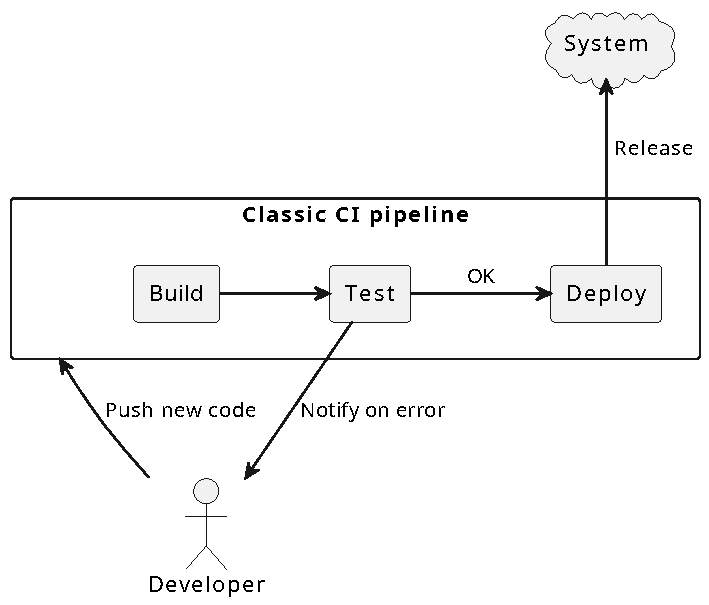
\includegraphics[width=0.6\textwidth]{figures/cicd-example.pdf}
	\caption{A classic example of a CI/CD pipeline.}
	\label{fig:ci-cd}
\end{figure}

To enable a pipeline, adequate tools and infrastructure are required. Over the last ten years, the CI/CD ecosystem has grown significantly,
and there are many tools available to support the pipeline.
As follow, a brief landscape of the most popular CI/CD tools is presented, showing the main features, the main advantages and disadvantages.

Jenkins is a free, open-source automation server that helps streamline the software development process by automating tasks such as building,
testing, and deploying code. It offers hundreds of plugins to support various technologies and tools, making it a highly versatile platform. Jenkins
is often used for continuous integration and continuous delivery (CI/CD) workflows, allowing developers to quickly and easily validate and release
code changes. The~\Cref{lst:jenkins-example} shows an example of a \emph{Jenkinsfile} written in Groovy syntax that builds a java project and
subsequently runs the tests.

In the example, the Jenkinsfile defines a pipeline with two stages: one for building the application using Maven, and one for testing it. This is
just a simple example of what can be achieved with Jenkins, but it demonstrates how it can help automate and streamline the software development
process.

\lstinputlisting[
	float=h,
	language=Kotlin,
	caption={A Jenkinsfile example.},
	label={lst:jenkins-example}
]{listings/jenkins-example}

\emph{GitHub Actions} is a powerful CI/CD platform integrated into GitHub that allows developers to automate their software development workflows.
With GitHub Actions custom workflows that run on specific events can be defined, such as code pushes, pull requests, and releases. Workflows are
defined using \emph{YAML} files and can include multiple steps, such as building and testing code, deploying to various environments, and more.

Here is a simple example of a GitHub Actions workflow that builds and tests a Java application:

\lstinputlisting[
	float=h,
	caption={A GitHub Actions workflow example.},
	label={lst:github-actions-example}
]{listings/gha-example.yaml}

In the~\Cref{lst:github-actions-example}, the workflow is triggered on pushes to the main branch and runs on an Ubuntu-based runner. The workflow
includes steps to check out the code, set up a Java environment, build the application, and run tests. With GitHub Actions, you can easily
automate and streamline your software development workflows, helping to improve efficiency and reduce errors.

An \emph{action} in the context of GitHub Actions is a pre-written, reusable piece of code that performs a specific task within a software development
workflow. These actions can be run as part of a workflow to automate tasks such as building code, testing it, deploying it, and more.

\paragraph*{}

The choice to use GitHub Actions to implement the CI/CD pipeline was made primarily for reasons of practicality and prior knowledge, but also because
it boasts a large community that supports and maintains the actions.
The pipeline is structured into three main jobs:

\begin{itemize}
	\item \textbf{Build}: the build job is responsible for running all the quality assurance tools, compiling the source code and generating the
	      artifacts
	\item \textbf{Test}: the test job runs all the unit tests and integration tests, and it is responsible to upload the artifacts on the
	      Maven Central repository and close the repository
	\item \textbf{Release}: the release job is responsible for releasing the artifacts on the Maven Central repository
\end{itemize}

All the aforementioned jobs are executed in parallel over three different operating systems: Windows, Linux and macOS.
The use of three different operating systems allows for verification that the framework is compatible with all the major operating systems and the relative
platforms, reducing the probability of errors on a specific platform.

When working with Kotlin multiplatform, the pipeline slightly changes, since the artifacts must be generated for each supported platform.
To achieve this, the pipeline is enriched with some additional jobs: the very first job is responsible for creating the staging repository on the
Maven Central repository, setting up the environment for a possible release. Then, are executed the build, test and release jobs for each platform.
A specific job is also added after the build job to close the staging repository on the Maven Central repository, and consequently, trigger the
checks over the repository. Finally, the release job is executed to release the artifacts on the Maven Central repository if needed
(see~\Cref{fig:ci-cd-pipeline}).

\begin{figure}[h]
	\centering
	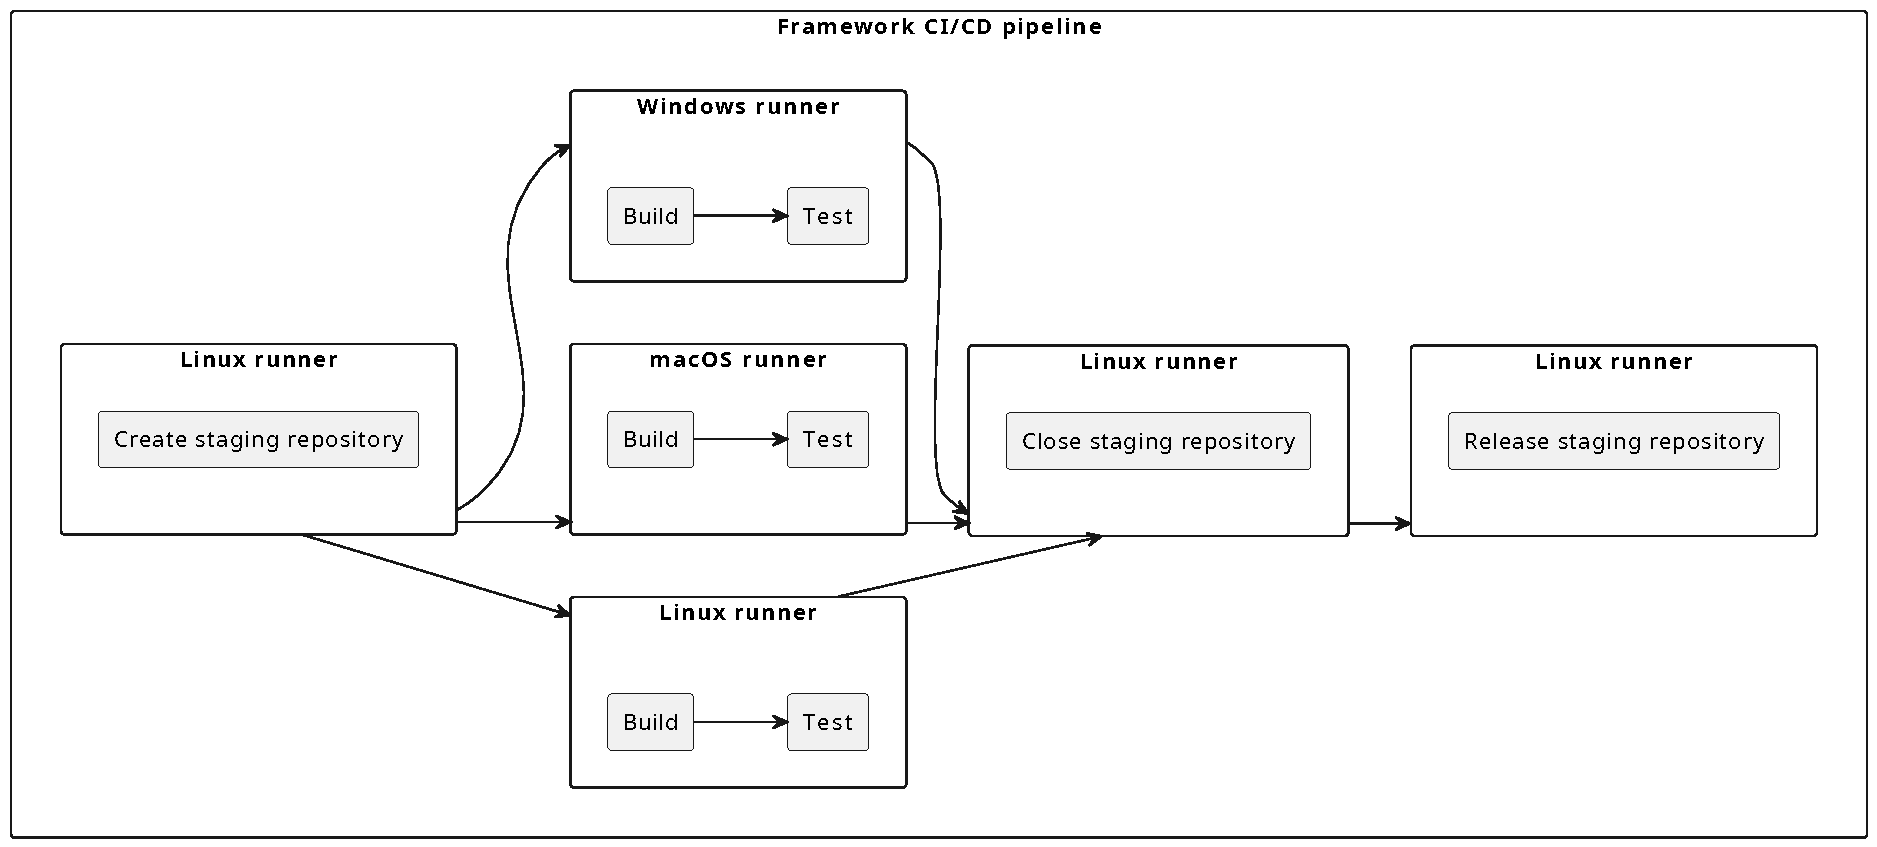
\includegraphics[width=\textwidth]{figures/framework-ci.pdf}
	\caption{The CI/CD pipeline of the framework.}
	\label{fig:ci-cd-pipeline}
\end{figure}

The rationale behind the choice of using a dedicated job for creating the staging repository is due the fact that the subsequent jobs are executed
in parallel over different OS, which means that they would create a different staging repository for each OS, leading to an unintended condition.
Using the aforementioned approach, the staging repository is created only once, and then, the subsequent jobs are executed over the same repository
by sharing the \emph{repository id}. In this way, the artifacts coming from different OS are uploaded to the same repository (using the repository id
generated before), and consequently, the release job releases all the artifacts on the Maven Central repository consistently.

Code maintenance is a key aspect of good project lifecycle management.
For this reason, tools such as \emph{renovate,} \emph{mergify} and \emph{semantic-release} have been used to automate these aspects.

Renovate is an automated tool that is used to manage and automate the process of updating
dependencies and keeping projects up-to-date. The Renovate Bot can be integrated into a project's code repository and configured to automatically
detect when updates are available and then create pull requests to implement the updates. This can help to streamline the process of keeping
dependencies up-to-date and reduce the risk of security vulnerabilities or compatibility issues.

Mergify is an automated tool that helps to manage and automate the process of merging pull requests in a code repository. The Mergify bot
can be integrated into a project's code repository and configured to automatically merge pull requests that meet specific criteria, such as passing
all required tests or receiving approval from a specified number of reviewers. This can help to speed up the code review process and reduce the
workload of maintainers, freeing them up to focus on more strategic tasks.

The semantic-release is a tool that automates the process of versioning and releasing software projects. It uses a specific commit message syntax to
determine the type of changes made in each commit message~\footnote{\url{https://www.conventionalcommits.org/en/v1.0.0/}} and automatically generates a new version number and make a
release based on those changes.
This helps to ensure that version numbers are consistently and accurately updated, reducing the risk of errors and allowing teams to
focus on more important tasks. Additionally, by automating the release process, semantic-release can help to speed up the development cycle and allow
teams to deliver new features and bug fixes to users more quickly and efficiently.

The joint use of these three tools on the one hand greatly speeds up the release and maintenance process of the code but on the other hand, should be
paid attention to the fact that since are automatic tools, they could cause unintended updates causing repercussions on the proper functioning of the
project, such as updating a dependency that modifies a public API thus making it incompatible with its use in the code. To minimize these scenarios,
an extensive and complete test suite should be set up, but also a CI/CD pipeline that intercepts similar a problem should be used; in this
way, maintainers are notified and they proceed with manual intervention to resolve the issue.

Therefore, all these details have been carefully attended to so that no situations arise that lead to inconsistencies or
incompatibilities in the code base: renovate is configured to open a pull request as soon as a new version of any dependency is available; mergify is
configured to merge automatically the PRs coming from Renovate which the status check is passed, and semantic-release is configured to make a
release only from the \emph{master} branch and if the previous jobs are completed successfully.

\section{Demo 1: Single Device Multiple Components}
\label{sec:demo-1}

With the first demo, a simple system was aimed at highlighting the main aspects of pulverization instantiated in a real physical scenario.
As a second goal, the demo aims to provide a reference on how it is possible to ``pulverize'' a device through the framework by also testing it in a
context closer to real use cases.

This demo models the following scenario: you want to monitor the moisture status of soil through a device
by sensing the moisture level of the soil and through a valve, set the water flow to properly adjust the desired moisture level.
This simple scenario involves several aspects of the pulverization: first, we find the concepts of sensor and actuator, which respectively serve to
acquire the soil moisture level and regulate water flow. Finally, the behavior specifies how the flow regulation should occur based on
the detected moisture. The~\Cref{fig:demo-1-system} shows the components defining the logical device.

\begin{figure}[h]
	\centering
	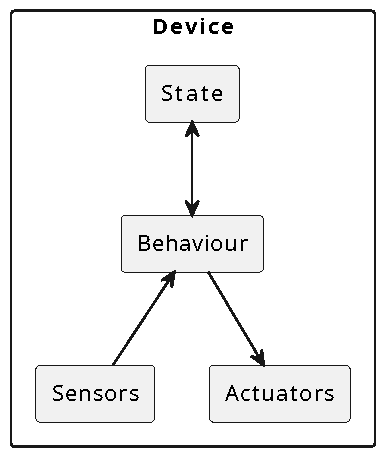
\includegraphics[width=0.4\textwidth]{figures/demo1-device.pdf}
	\caption{Decomposition of the moisture device into the pulverization components showing the interaction between them.}
	\label{fig:demo-1-system}
\end{figure}

The physical system is composed of three devices: two embedded systems used respectively for moisture sensing and water flow regulation and a server
which represents the infrastructure where the pulverized system runs.
Two \textbf{ESP32}~\footnote{\url{https://www.espressif.com/en/products/socs/esp32}} boards are used to implement the sensor component and the
actuator component. The primary rationale behind selecting these boards is their cost-effectiveness and ease of use. Additionally, they come equipped
with a Wi-Fi module, facilitating communication with the pulverization platform.

\begin{figure}[h]
	\centering
	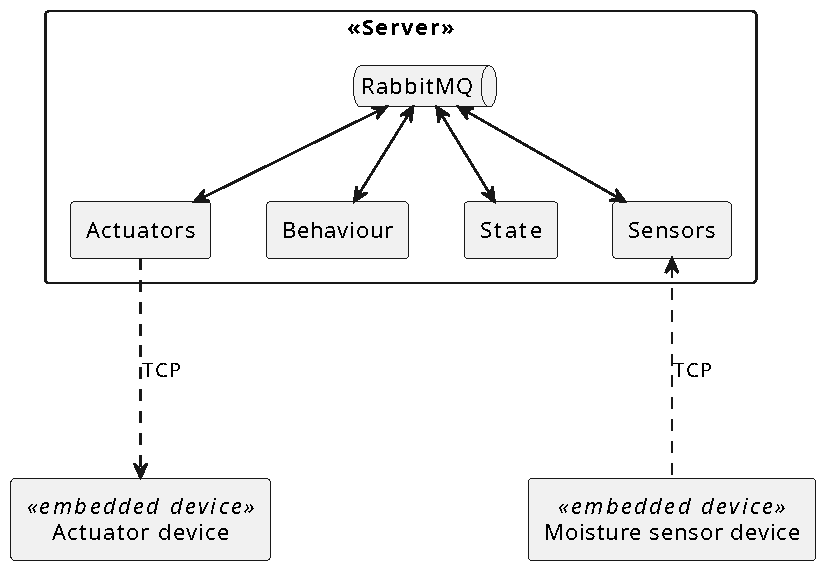
\includegraphics[width=0.7\textwidth]{figures/demo1-physical.pdf}
	\caption{Physical system architecture where are reported the communication between the components and the server.}
	\label{fig:demo-1-physical-system}
\end{figure}

In~\Cref{fig:demo-1-physical-system} is reported the physical system architecture where are reported the communication between the components and the
server.

The multiplatform nature of the framework allows the execution of each ``pulverized component'' on different architectures.
But at the time of writing, even if the number of supported architectures in Kotlin multiplatform is quite high, the framework does not support the
\textbf{Xtensa}~\footnote{\textbf{Xtensa} is a configurable and extensible processor architecture developed by Tensilica, now owned by Cadence Design Systems. It is designed to meet the unique requirements of a wide range of applications and systems, from low-power IoT devices to high-performance computing systems.}
architecture used by the ESP32 boards.

This limitation is solved as follows: we can think of the \emph{sensor component} as acting as a kind of proxy by collecting data from
the embedded device. In this way, the firmware that will control the board will be written in a language that supports the Xtensa architecture and
will provide a communication mechanism with the \emph{sensor component} that will simply forward the received message to other components.
As can be seen, the framework is extremely flexible, allowing it to accommodate limitations such as the one described above.

In this specific case, the limitation described above is solved by writing the \textbf{ESP32} firmware in \emph{Rust} (a language that supports the
Xtensa architecture) and implement the communication with the \emph{sensor component} using a TCP socket. The \emph{sensor component} is
implemented using the framework interface where a TCP socket is opened to listen for incoming messages from the embedded device.
On each received message, the sensor's value is extracted and saved in a local state; in this way, on each \texttt{sense} method call,
the last received value from the embedded device is returned.
This simple workaround allows the use of the pulverization framework also in devices that do not support the Kotlin multiplatform architecture.
The explanation of the limitation was made using the \emph{sensor component} as an example, but the same principle was applied to the
\emph{actuator component}, so again via TCP socket, a message is sent to the embedded device for opening or closing the valve.

As follow, are reported the main relevant details of the implementation of this demo.
As discussed above, the device has four components: \emph{sensor}, \emph{actuator}, \emph{behavior} and \emph{state};
the~\Cref{lst:demo-1-configuration} shows the configuration of the logical device where the \emph{sensor} and \emph{actuator} components are
deployed into two devices, and the \emph{behaviour} and \emph{state} components are deployed into the server.

\lstinputlisting[
	float=ht,
	language=Kotlin,
	label={lst:demo-1-configuration},
	caption={Configuration of the logical device named ``moisture-device''.}
]{listings/demo-1-config.kt}

The \emph{behaviour} component defines the logic of the device: retrieve the moisture level from the \emph{sensor} component and, if the moisture level is below a threshold, open the valve using the \emph{actuator} component. The \emph{state} component is used to store the moisture level.
The~\Cref{lst:demo-1-behaviour} shows the implementation of the \emph{behaviour} component.

Finally, the three deployment units are defined and containerized using Docker. In particular, a \emph{RabbitMQ} container is used to provide the
communication between the components, while the other three containers are used to run the \emph{sensor}, \emph{actuator} and \emph{behaviour}
components. Since the three components are deployed into three different containers, these may be deployed on different machines without affecting
the execution of the logical device.

The test of the demo was conducted on a local Linux machine running the four containers and the two ESP32 boards. All the containers are deployed
using \emph{Docker Compose}.
The two ESP32 boards are connected to the same Wi-Fi network and the \emph{sensor} and \emph{actuator} components are configured to connect to the
respective container using the IP address of the machine where the container is running.
Finally, the increase and decrease of soil moisture were simulated by verifying that the valve opened and closed properly to maintain the desired
level of moisture in the soil.

\lstinputlisting[
	float=ht,
	language=Kotlin,
	label={lst:demo-1-behaviour},
	caption={Implementation of the \emph{behaviour} component for the demo 1.}
]{listings/demo-1-behaviour.kt}

\section{Demo 2: Multi Devices Multi Components}
\label{sec:demo-2}

Demo 2 aims to represent a more complex scenario than the previous one, involving multiple devices and enabling communication between them.
Also, we want to introduce more types of devices and show how they are supported by the framework.
This demo gets even closer to real scenarios involving multiple types of devices and where communication between them is a prerequisite.

This demo tries to replicate the hot-warm-cold game using two types of devices: an embedded device that needs to be found and many smartphones that
need to find it. The smartphones connect to the embedded device via Bluetooth, through which they determine its distance and communicate
this information with other smartphones. The embedded device receives the information on the distances of the smartphones and sets a light intensity
of an LED proportional to the proximity of the smartphones to it. Thus, the closer the smartphones are to the embedded device, the brighter the led
will emit; while the farther away the smartphones are, the less light will be emitted.
Each smartphone sends its distance to all other smartphones and simultaneously receives the distance of all other smartphones from the embedded
device. Sharing distance information is intended to test inter-device communication while simultaneously providing clues as to where the device that
needs to be found is located so that it can be found more quickly.

A Raspberry PI was used as the embedded device since it has both Wi-Fi and Bluetooth. The ESP32 was not chosen, as in the previous demo, because it
has hardware limitations that prevent Bluetooth and Wi-Fi from being used simultaneously. As for smartphones, Android smartphones were used, thus
allowing the framework to be tested on this platform as well.

When designing a pulverized system, it is good to represent the system from two different viewpoints: a viewpoint that captures the logical level
of the interactions between logical devices (see~\Cref{fig:demo-2-logical-diagram}) and a physical viewpoint that shows how the system is deployed in
the infrastructure (see~\Cref{fig:demo-2-physical-diagram}).

\Cref{fig:demo-2-logical-diagram} shows the network topology and how devices are tied together. This level of abstraction is what should be used by
the user who intends to implement the system by exploiting the pulverization framework: he or she does not have to worry about infrastructure or
deployment aspects; how communications take place is handled directly by the framework. This greatly simplifies the development of the system. How
then the system is deployed in the infrastructure is depicted in~\Cref{fig:demo-2-physical-diagram}, which shows at the physical level where
components are executed and how intra-component communications of each device take place. Moreover, are depicted all the physical devices involved in
the system.

\begin{figure}[h]
	\centering
	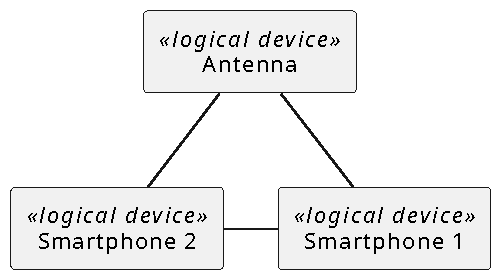
\includegraphics[width=0.6\textwidth]{figures/demo2-logical-device.pdf}
	\caption{Logical diagram of the connection between the logical devices.}
	\label{fig:demo-2-logical-diagram}
\end{figure}

\begin{figure}[h]
	\centering
	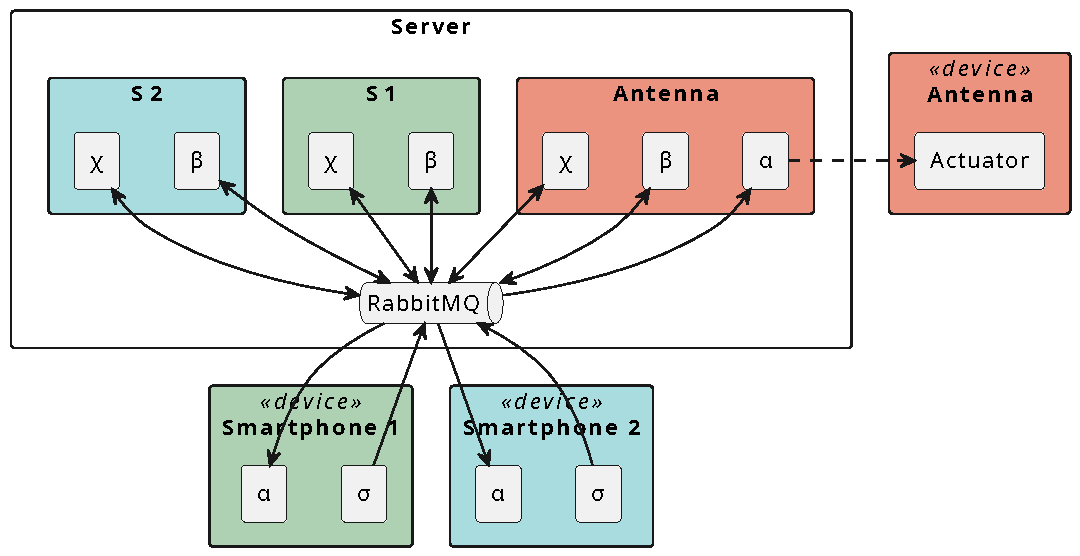
\includegraphics[width=\textwidth]{figures/demo2-physical.pdf}
	\caption{Physical diagram of the connection between the logical devices.}
	\label{fig:demo-2-physical-diagram}
\end{figure}

Design choices for the implementation of the demo are explained below. The demo is divided into four main modules:

\begin{itemize}
	\item \textbf{Android application:} in this module is implemented the mobile application that runs on smartphones
	\item \textbf{Raspberry PI firmware:} this module implements the firmware that runs on the Raspberry PI
	\item \textbf{Common module:} this module contains the common code shared between the \emph{Platform} and \emph{Android application} modules
	\item \textbf{Platform module:} this module contains the code that runs all the devices' components logics.
\end{itemize}

The \emph{common module} contains the code shared between the \emph{platform} and \emph{android application} modules. In particular, it contains
the implementation of each component like the \emph{behaviour, sensors} and \emph{actuators} components, either for the embedded device and the
smartphones. The reason why all the components are implemented in the same module is because they can be reused whenever a new device is added to the
system. In this way, the specific device should not implement its specific version of the component but instead reuse the one already implemented.

The android application is structured as follows: during the \emph{initialization} stage the pulverization platform with its components is
initialized and the \emph{Bluetooth LE} module configured. Then, a user interface is shown to the user, which allows them to start the system by
providing the IP of the machine where the platform is running and the device id. Once the user starts the system, the \emph{Bluetooth LE} module
starts scanning for nearby devices and, when the embedded device is found (the Raspberry PI), the \emph{Bluetooth LE} module connects to it and
starts sending the distance information to all its neighbours. At the same time, the application listen for incoming messages from the neighbours
and shows their distance on the screen.

The Raspberry PI firmware is structured as follows: first of all, the \emph{Bluetooth LE} module is configured as a server and starts the
advertising process, so that all the nearby devices can connect to it. Then, a TCP socket is opened toward the \emph{actuator component} deployed
on the server. Once the connection is established, all the incoming messages are collected. The message contains a decimal value between $0$ and $1$
that respectively means LED turned off and LED turned on; all the intermediate values are used to set the LED intensity.

Finally, the \emph{Platform} module defines for each logical device in the system all its deployment units. In particular, runs the
\emph{behaviour, sensors} and \emph{actuators} components for each smartphone and the \emph{behaviour} and \emph{actuators} components for the
embedded device.

The system was dockerized and deployed using docker compose. The system, once started, was tested by using two smartphones that were
continuously moved around the room to observe how it varied the LED intensity accordingly. The conducted test did not reveal any anomalies or
malfunctions, except for some inaccuracies in the calculation of the distance of the devices from the Bluetooth antenna due to signal
fluctuations.

One notable test that has been conducted involves simulating a device failure and observing how the system reacts to this condition.
The failure of a device was simulated by disconnecting it from the network.
As soon as the device was disconnected from the network, the system continued to operate as expected. Devices that were still active, store the last
message received from that device and thus did not alter their behavior. When the device returns operational in the network, then it will start
sending the newly updated data to its neighbors again, which will then update the information about that device's distance from the antenna.

In conclusion, this demo brought out the effectiveness of the framework in clearly separating business logic development from infrastructural and
deployment aspects, highlighting how more complicated systems are achievable through the pulverization framework. Again, it highlighted how a failure
of one component does not preclude the system's operation.

This demo can be extended by going to improve the calculation of the distance of the devices from the antenna, for example, by implementing a filter
that reduces the noise in the signal acquisition producing more stable and truthful values. Another interesting aspect to analyze may be to have some
smartphones with all components running on them, while other smartphones have the behavior running in the cloud, thus observing that the overall
behavior does not change as the deployment structure changes.

\section{Current framework limitations}
\label{sec:framework-limitations}

At present, the framework has some limitations: dynamics and support for different protocols are some examples of shortcomings.
The goal of this section is therefore to provide an overview of the main shortcomings of the framework by going on to examine in what contexts these,
if implemented, could solve certain problems.

\subsection{Dynamics}
\label{sec:dynamics}

By dynamism, in this context, we mean the ability of the framework to be able to dynamically relocate pulverized components in the infrastructure.

At present, the framework does not handle this aspect: the deployment structure is defined a priori and remains so throughout the life of the
executed system. Although dynamism is a key aspect in pulverization, it was decided to focus more on good domain modeling to build a solid foundation
on which the framework can be extended, rather than implementing as many aspects as possible running the risk of creating a rigid framework that is
not very extensible and difficult to use.

\subsection{Multi-protocols}
\label{sec:multi-protocols}

The management of multiple protocols to enable intra-component communication is an important aspect since pulverization can involve a large number of
heterogeneous devices that have different computational and communication capabilities.

For this reason, the choice of one protocol over another is not mutually exclusive, but it may be appropriate, for example, to provide
multiple protocols that are used in the pulverized system. Again, you might be dealing with devices that do not support certain protocols, or you are
in a situation where you want to use a very lightweight protocol (e.g. MQTT) for devices with very low computational resources and instead use a
higher-performance protocol for those parts of the system with high computational power.

At the time of writing, the only protocol implemented to enable intra-component communication is RabbitMQ as it represents a good compromise between
ease of use, performance and adoption.

Adoption of additional protocols would increase the framework's potential to be used in many contexts with strong device heterogeneity.
%----------------------------------------------------------------------------------------

% Conclusions ---------------------------------------------------------------------------
\chapter{\conclusionsname}
\label{chap:conclusions}

The increasing use of Internet of Things (IoT) devices and the resulting large amounts of data being produced present significant challenges for
cloud computing. While cloud computing has proven effective for many applications, it may not always be suitable for real-time constraints and
handling data from IoT devices.

Fog computing offers a promising solution by providing a computing model that sits between IoT devices and the cloud,
allowing for the collection, aggregation, and processing of data using a hierarchy of computing power. Combining fog computing with the cloud can
reduce data transfers and communication bottlenecks, as well as contribute to reduced latencies. However, realizing systems that operate in the
edge-cloud continuum is a complex challenge due to the heterogeneity of devices and dynamic requirements of today's systems.

Various approaches have been proposed to address these challenges, including self-organizing systems and methodologies such as osmotic computing and
DR-BIP. The orchestration of distributed applications requires careful management of the underlying infrastructure to enable the reuse of design
elements across different scenarios.

The thesis focuses more specifically on the pulverization approach: a framework that breaks the system behaviour into small computational pieces that
are continuously executed and scheduled in the available infrastructure.
In this way, the business logic of a system is neatly separated from infrastructure or deployment concerns enabling the concept of
\emph{deployment independent} systems.
Reuse and independency from the deployment are the two main pillars of the pulverization approach, by which the framework aims to enable the
deployment of systems in the edge-cloud continuum.

The main contribution of the thesis is the development of a framework that leverages the pulverization approach to deploy Cyber-Physical Systems.
The framework aims to lay the groundwork for closing the gap between the simulation of these systems and their deployment by exploiting the
pulverization methodology.

The framework is built trying to maintain ease of use, modularity, and extensibility by modeling well the foundational concepts of pulverization over
which the framework can be extended and improved.

Several technology solutions were examined that could support cross-platform targets allowing the framework to be used seamlessly across different
platforms and architectures. Kotlin multiplatform was identified as a suitable technology for the development of the framework since it has a wide
range of supported architectures.

The most significant implementation details and technology challenges that were faced during the development of the framework and what solutions were
employed to achieve it were reported.

Finally, topics such as testing and validation were covered by showing what strategies were used to validate the operation of the framework, as well
as significant demos were developed to show how the framework works in different contexts, each of which brings with it peculiar characteristics that
go to corroborate the proper operation and effectiveness of the framework.

From using the framework, it seemed evident that deployment aspects never appear during system implementation, leading to the advantage of focusing
most efforts on development, delegating infrastructure and communication aspects to the framework. In addition, it was apparent how the reusability
of the developed components is easily achieved by design: this leads to the same component being able to be reused in different deployment strategies
in different infrastructures, making it flexible to changes in how it is deployed.

\section{Future Works}
\label{sec:future-works}

The framework is still in its early stages of development and there is still a lot of work to be done to make it more robust and complete. The
following are some of the topics that could be explored in future work.

Due to the heterogeneity of the devices that can be used in the edge-cloud continuum, the framework should be able to support different
communication protocols. This would allow the framework to be used in a wider range of scenarios allowing the use of different communication
protocols based on device capabilities. Moreover, this work can be extended to support different communication protocols at the same time to
opportunistically exploit the best protocol for the actual system requirements or quality of services.

Dynamics is a key aspect of the edge-cloud continuum, and the framework should be able to support dynamic changes in the system. This would allow
the framework to be used in scenarios where the system is subject to changes in the number of devices, the number of resources, or opportunistically
exploit the best deployment strategy for the actual system.

Currently, to deploy the system, some manual steps such as containerizing the deployment units that will then run in the available infrastructure
must be performed. Automating this process can reduce the time to deploy the system by reducing the likelihood of error in container deployment.
As a consequence, it makes sense to study how downstream of containerization, containers can be automatically deployed into the infrastructure
through DevOps (CI/CD) methodologies.

\paragraph*{}

With this thesis, I brought in research topics and problems such as pulverization. It was motivating to delve into and understand the
concepts of pulverization and carry them into the implementation of a framework. Equally satisfying was seeing the framework work in different
contexts and understanding how it could be evolved in the future. This experience allowed me to study the literature and understand what
related work has already drawn useful insights from it to implement the framework.
In addition, this thesis allowed me to delve into the Kotlin ecosystem in its multiplatform version by understanding how this technology may be
suitable to support the implementation of the framework.

\todo{Vedere se aggiungere altro}

%----------------------------------------------------------------------------------------

%----------------------------------------------------------------------------------------
% BIBLIOGRAPHY
%----------------------------------------------------------------------------------------

%\nocite{*} % uncomment this to show all the references in the .bib file
% \bibliographystyle{plain}
% \bibliography{bibliography}
\printbibliography

\end{document}
